%%%%%%%%%%%%%%%%%%%%%%%
% Dissertation Defense
%%%%%%%%%%%%%%%%%%%%%%%

% Title Slide
{\setbeamertemplate{background canvas}{
\tikz[remember picture,overlay]
	\node[opacity=0.3] at (current page.center) {
	\includegraphics[width=\paperwidth,
	height=\paperheight]{images/curve2.png}};} 

\begin{frame}[plain] \vspace{1.8cm}
\begin{center}
\phantom{.}\par
	{\Large\color{UniOrange} \textsc{Torsion Subgroups of}  \textsc{Rational Elliptic Curves over}  \textsc{Odd Degree Galois Fields}} \par\vspace{0.2cm}

	{\large\color{UniGray}\textit{Caleb McWhorter} \par
	\textit{Syracuse University}} \par\vspace{1.8cm}
	
	{\small\color{UniGray} April 22, 2021}
\end{center}
\end{frame}
}





%%%%%%%%%%%
% Background
%%%%%%%%%%%

% Definition
\begin{frame}[plain]
\begin{dfn}[Arithmetic Geometry]
Arithmetic Geometry is the study of `interesting' equations in Number Theory (Diophantine equations) using techniques from Algebraic Geometry.
\end{dfn}
\end{frame}



% Examples
\begin{frame}[plain] \frametitle{Examples}
\begin{itemize}
\item Is there a rational number such that its cube is two larger than its square?
	\[
	x^3= x^2 + 2
	\]

\item Is the sum of squares ever a square? 
	\[
	y^2= \dfrac{x (x + 1) (2x + 1)}{6}
	\]

\item Are there squares two less than a cube? 
	\[
	y^2= x^3 - 2
	\]

\item What numbers are the sum of two (or more) cubes? 
	\[
	x_1^3+x_2^3+\cdots+x_n^3= N
	\]
\end{itemize}
\end{frame}








% Fermat's Last Theorem
\begin{frame} \frametitle{Fermat's Last Theorem}

\begin{thm}[{\small Fermat's Last Theorem; Wiles, 1994; Taylor-Wiles, 1995}]
If $n > 2$, there are no (nontrivial) integer solutions to the equation
	\[
	x^n + y^n= z^n
	\]
\end{thm} \pspace

\begin{quote}
Cubum autem in duos cubos, aut quadratoquadratum in duos quadratoquadratos \& generaliter nullam in infinitum ultra quadratum potestatem in duos eiusdem nominis fas est dividere cuius rei demonstrationem mirabilem sane detexi. Hanc marginis exiguitas non caperet.
\end{quote} \pspace

``I have a truly marvelous proof of this, which these margins are too narrow to contain.''
\end{frame}





% Congruent Number Problem
\begin{frame} \frametitle{Congruent Number Problem}
\emph{Congruent Number:} We call an integer $n$ congruent if it is the area of a rational right triangle. \pspace

This is equivalent to finding a rational triplet $(x,y,z)$ with\dots
	\[
	x^2 + y^2= z^2 \quad \text{ and } \quad n= \dfrac{xy}{2}.
	\] \pspace
Furthermore, this is equivalent to finding a rational solution $(x,y)$ to
	\[
	y^2= x^3 - n^2 x
	\]
\end{frame}



% Examples
\begin{frame}
\begin{ex}
\begin{itemize}
\small
\item 6 is congruent: $3^2 + 4^2= 5^2$ and $\dfrac{3(4)}{2}= 6$
\item 5 is congruent: $(3/2)^2 + (20/3)^2= (41/6)^2$ and $\dfrac{(3/2)(20/2)}{2}= 5$
\item 1 is \emph{not} congruent (due to Fermat) 
\item 157 is congruent (due to Zagier):
	\[
	\begin{aligned}
	x&= \dfrac{411340519227716149383203}{21666555693714761309610} \\
	y&= \dfrac{6803298487826435051217540}{411340519227716149383203} \\
	z&= \dfrac{224403517704336969924557513090674863160948472041}{8912332268928859588025535178967163570016480830}
	\end{aligned}
	\]
\end{itemize}
\end{ex}
\end{frame}





% Isosceles Triangle Problem
\begin{frame} \frametitle{Isosceles Triangle Problem}
{\itshape Does there exist a rational right triangle and a rational isosceles triangle that have the same area and the same perimeter?} \pspace

If yes, we can find $t, u \in \Q$, $0 < t < 1$, $0 < u < 1$, and $k > 0$. 
	
	\begin{figure}[!ht]
	\centering
	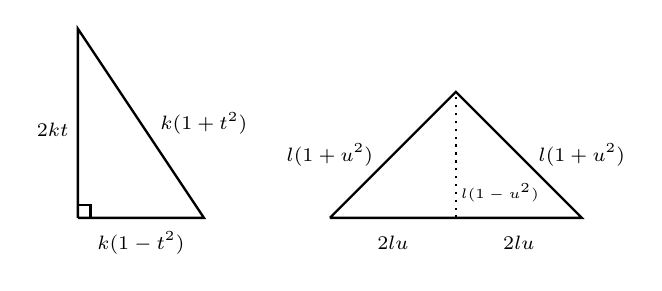
\begin{tikzpicture}[scale=0.8]
	\draw[line width=0.03cm] (0,0) -- (0,3) -- (2,0) -- (0,0);
	\draw[line width=0.03cm] (0,0.2) -- (0.2,0.2) -- (0.2,0);
	\node at (1,-0.4) {\scriptsize$k(1-t^2)$};
	\node at (-0.4,1.4) {\scriptsize$2kt$};
	\node at (2.0,1.5) {\scriptsize$k(1+t^2)$};
	
	\draw[line width=0.03cm] (4,0) -- (6,2) -- (8,0) -- (4,0);
	\draw[line width=0.03cm,dotted] (6,0) -- (6,2);
	%\draw[line width=0.03cm] (5.85858,1.85858) -- (6,1.71716) -- (6.14142,1.85858);
	\node at (4,1) {\scriptsize$l(1+u^2)$};
	\node at (8,1) {\scriptsize$l(1+u^2)$};
	\node at (5,-0.4) {\scriptsize$2lu$};
	\node at (7,-0.4) {\scriptsize$2lu$};
	\node at (6.7,0.4) {\tiny$l(1-u^2)$};
	\end{tikzpicture}
	\end{figure} 
With even more algebra, this is the same as finding a rational solution $(x,y)$ to 
	\[
	y^2= x^6 + 12x^5 - 32x^4 + 52x^2 - 48x + 16
	\]
\end{frame}





% Result
\begin{frame}[plain]
\begin{thm}[Hirakawa, Matsumura 2018]
Up to similitude, there exists a unique pair of rational right triangles and a rational isosceles triangle which have the same perimeter and the same area. The unique pair consists of the right triangle with side $(377,135,352)$. and isosceles triangle with sides $(366,366,132)$. 
\end{thm}
\end{frame}





% Introduction
\begin{frame}[plain]
\footnotesize
\begin{ques}
Let $F(x_1,x_2,\ldots,x_n) \in \Q[x_1,\ldots,x_n]$. Consider the equation $F(x_1,\ldots,x_n)= 0$.
\begin{itemize}
\item When are there rational solutions?
\item If there are rational solutions, how many are there?
\item Can we find/parametrize all the rational solutions?
\item What about integer solutions?
\end{itemize}
\end{ques}
\end{frame}





% Rational Roots Theorem
\begin{frame}[plain]
\begin{thm}[Rational Roots Theorem]
Let $f(x)= a_n x^n + a_{n-1} x^{n-1} + \cdots + a_0$, where $a_i \in \Z$ and $a_0,a_n \neq 0$. Then the only rational solutions to $f(x)=0$ have $x= p/q$, where $p$ is an integer factor of $a_0$ and $q$ is an integer factor of $a_n$. 
\end{thm}
\end{frame}





% Case of Two Variables
\begin{frame}[plain] \frametitle{What about two variables?}
$F(x,y)= ax + by + c \in \Q[x,y]$ \pspace
	\[
	ax + by + c = 0 
	\] \pspace 

\begin{itemize}
\item Infinitely many rational points. \pspace
\item We can parametrize these solutions. \pspace
\item Integer solutions if $\gcd(a,b)$ divides $c$. If so, infinitely many. 
\end{itemize}
\end{frame}





% Conics
\begin{frame}[plain] \frametitle{What about Degree Two?}

$F(x,y)= ax^2+bxy + cy^2 + ex+fy+h \in \Q[x,y]$. \pspace
	\[
	ax^2+bxy + cy^2 + ex+fy+h= 0
	\] \pspace

\begin{itemize}
\item  These are the conic sections: circles, ellipses, parabolas, hyperbolas, and degenerate cases like a point or pair of lines. 

\item We want our curves to be smooth, i.e. there is no solution (over $\C^2$) to
	\[
	F(x,y)= \dfrac{\partial F}{\partial x}(x,y)= \dfrac{\partial F}{\partial y}(x,y)= 0
	\]
\end{itemize}
\end{frame}





% Examples
\begin{frame}[plain,t] \frametitle{Finding Rational Points}
	\[
	x^2 + y^2 = 1 
	\] \vfill
	\[
	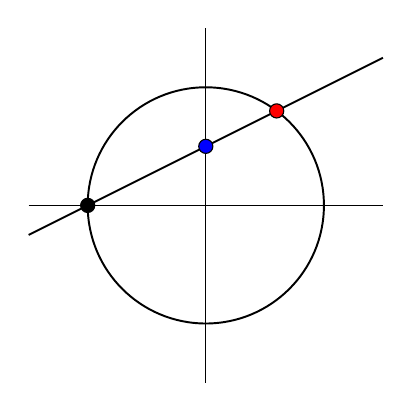
\begin{tikzpicture}[scale=1.5]
	\draw (-1.5,0) -- (1.5,0);
	\draw (0,-1.5) -- (0,1.5);

	\draw[line width=0.7] (-1.5,-0.25) -- (1.5,1.25);
	\draw[line width=0.7] (0,0) circle (1);
	
	\draw[fill=black] (-1,0) circle (0.06);
	\draw[fill=blue] (0,0.5) circle (0.06);
	\draw[fill=red] (0.6,0.8) circle (0.06);
	\end{tikzpicture}
	\] \vfill
	\[
	C(\Q)= \{ (-1,0) \} \cup \left\{ \left(\dfrac{1-t^2}{1+t^2}, \dfrac{2t}{1+t^2} \right) \colon t \in \Q \right\}
	\] \pspace
\end{frame}





% Hilbert's 10 Problem
\begin{frame}[plain] \frametitle{Hilbert's 10\textsuperscript{th} Problem}

\begin{table}[!ht]
\begin{tabular}{|c|c|c}  \cline{1-2}
Ring & Hilbert's 10\textsuperscript{th} & \hspace{1cm} \llap{\tikz[remember picture]\node (top node){};\hspace*{1em}} \\ \cline{1-2}
$\C$ & \cmark \\
$\R$ & \cmark \\
$\F_q$ & \cmark \\
$p$-adic fields & \cmark \\
$\F_q(\!(t)\!)$ & ? \\
Number Fields & ? \\
$\Q$ & ? \\
Global Function Fields & \xmark \\
$\F_q(t)$ & \xmark \\
$\C(t)$ & ? \\
$\C(t_1,\ldots,t_n)$ & \xmark \\
$\R(t)$ & \xmark \\
$\O_K$ & $\approx$? \\
$\Z$ & \xmark & \hspace{1cm} \llap{\tikz[remember picture]\node (bottom node){};\hspace*{1em}} \\ \cline{1-2}
\end{tabular}
\end{table}

\begin{tikzpicture}[remember picture, overlay]
\draw[->,very thick] (top node) -- (bottom node) node[midway,sloped,right,yshift=2ex] {\hspace{-3.1cm}\text{increasing arithmetic complexity}};
\end{tikzpicture}
\end{frame}





% Higher Curves
\begin{frame}[plain]
\ctext{What about higher degree curves?}
\end{frame}





% Falting's Theorem
\begin{frame}[plain]
\begin{thm}[Mordell, 1922; Faltings, 1983]
If $C$ is a curve over $\Q$ of genus $g \geq 2$, then $C$ has at most finitely many rational points. 
\end{thm}
\end{frame}





% Interesting Case
\begin{frame}[plain]
\ctext{Interesting Case of Cubic Equations}
\end{frame}





% Quote
\begin{frame}[plain] 
	\begin{minipage}{0.2\textwidth}
 	\begin{figure}[h]
	\centering
	\fbox{\includegraphics[width=1\textwidth]{images/mordell.jpg}} \par
	{\small 1888--1972}
	\end{figure}
	\end{minipage}%
	\begin{minipage}{0.8\textwidth}
	\begin{center}
	{\itshape ``Mathematicians have been familiar with very few questions for so long a period with so little accomplished in the way of general results, as that of finding the rational [points on elliptic curves].''} \\
	 \phantom{x}\hfill-- L.J. Mordell, 1922
	\end{center}
 	\end{minipage}
\end{frame}





% General cubic to elliptic
\begin{frame}[plain] \frametitle{Elliptic Curves}
\footnotesize
Starting with a general homogeneous polynomial of degree 3 in three variables, we can reduce down to an elliptic curve in Weierstrass form:
	\[
	y^2 + a_1 xy + a_3y = x^3 + a_2 x^2 + a_4 x + a_6
	\] \pspace 

\begin{itemize}
\item Make the substitution $y \mapsto y + \dfrac{a_1 x+a_3}{2}$.
\item Obtain $y^2= x^3+ a_2' x^2 + a_4' x + a_6'$
\item Make the substitution $x \mapsto x + \dfrac{a_2'}{3}$
\end{itemize} \pspace 
	\[
	\text{Elliptic Curve: } E= E_{A,B}: y^2 = x^3 + Ax + B
	\] \pspace

\begin{itemize}
\item Require $\Delta:= -16(4A^3+27B^2) \neq 0$.
\item $E(\Q)$ could be empty, finite, or infinite. 
\end{itemize}
\end{frame}





% Examples 
\begin{frame}[plain]
	\begin{figure}[h]
	\centering
	\begin{subfigure}{0.45\textwidth}
	\includegraphics[width=\textwidth]{images/ec2.eps}
	\caption*{$y^2=x(x^2+1)$}
	\end{subfigure}
	%
	\begin{subfigure}{0.45\textwidth}
	\includegraphics[width=\textwidth]{images/ec1.eps}
	\caption*{$y^2=x^3-x+1$}
	\end{subfigure}
	\end{figure}
\end{frame}





% Examples
\begin{frame}[plain]
	\begin{figure}
	\centering
	\begin{subfigure}{0.45\textwidth}
	\includegraphics[width=\textwidth]{images/ec3.eps}
	\caption*{$y^2=x^2(x+2)$}
	\end{subfigure}
	\begin{subfigure}{0.45\textwidth}
	\includegraphics[width=\textwidth]{images/ec4.eps}
	\caption*{$y^2= x^3$}
	\end{subfigure}
	\end{figure}
\end{frame}





% Addition law
\begin{frame} \frametitle{\href{https://cgmcwhor.expressions.syr.edu/wp-content/uploads/2019/10/curve.mp4}{\textcolor{white}{Addition Law (Chord-Tangent Law)}}}
	\begin{figure}[h]
	\centering
	\includegraphics[width=0.65\textwidth]{images/ec_add.eps}
	\end{figure}
\end{frame}





% Points of Finite Order
\begin{frame} \frametitle{Points of Finite Order}
	\begin{figure}[!ht]
	\centering
	\includegraphics[width=0.6\textwidth]{images/ec5.eps}
	\end{figure}
\end{frame}





% EC Definition
\begin{frame}[plain]
\footnotesize
\begin{dfn}[Elliptic Curve]
An elliptic curve is\dots
\begin{itemize}
\item A nonsingular projective curve of genus 1. \pspace
\item An abelian variety of dimension 1. \pspace
\item A nonempty smooth variety, $V(F)$, with $\deg F=3$. \pspace
\item A compact Riemann surface of genus 1. \pspace
\item The set $\{(x,y) \colon y^2= x^3 + Ax + B, -16(4A^3+27B^2) \neq 0 \}$ $\cup \{\infty\}$ with an addition law given by the chord-tangent law. 
\end{itemize}
\end{dfn}
\end{frame}





% Structure of E
\begin{frame}[plain]
\ctext{What is the Group Structure?}
\end{frame}





%%%%%%%%%%%
% Mordell-Weil
%%%%%%%%%%%

% Mordell 
\begin{frame}
	\begin{thm}[Mordell, 1922]
	Let $E/\Q$ be an elliptic curve. Then the group of $\Q$-rational points on $E$, denoted $E(\Q)$, is a finitely generated abelian group. In particular,
		\[
		E(\Q) \cong \Z^{r_\Q} \oplus E(\Q)_\tors,
		\]
	where $r_\Q \geq 0$ is the rank of $E$ and $E(\Q)_\tors$ is the torsion subgroup.
	\end{thm}
	\begin{figure}[h]
	\centering
	\begin{subfigure}{0.3\textwidth}
	\captionsetup{labelformat=empty}
	\centering
	\fbox{\includegraphics[width=0.8\textwidth]{images/mordell.jpg}}
	\caption{Louis J. Mordell}
	\end{subfigure}
	%
	\phantom{
	\begin{subfigure}{0.3\textwidth}
	\captionsetup{labelformat=empty}
	\centering
	\fbox{\includegraphics[width=0.74\textwidth]{images/weil.jpg}}
	\caption{Andr\'e Weil}
	\end{subfigure}
	%
	\begin{subfigure}{0.3\textwidth}
	\captionsetup{labelformat=empty}
	\centering
	\fbox{\includegraphics[width=0.8\textwidth]{images/neron.png}}
	\caption{Andr\'e N\'eron}
	\end{subfigure}
	}
	\end{figure}
\end{frame}





% Mordell - Weil
\begin{frame}
	\begin{thm}[Mordell-Weil, 1928]
	Let $K$ be a number field, and let $A/K$ be an abelian variety. Then the group of $K$-rational points on $A$, denoted $A(K)$, is a finitely generated abelian group. In particular,
		\[
		A(K) \cong \Z^{r_K} \oplus A(K)_\tors,
		\]
	where $r_K \geq 0$ and $A(K)_\tors$ is the torsion subgroup.
	\end{thm}
	\begin{figure}[h]
	\centering
	\begin{subfigure}{0.3\textwidth}
	\captionsetup{labelformat=empty}
	\centering
	\fbox{\includegraphics[width=0.8\textwidth]{images/mordell.jpg}}
	\caption{Louis J. Mordell}
	\end{subfigure}
	%
	\begin{subfigure}{0.3\textwidth}
	\captionsetup{labelformat=empty}
	\centering
	\fbox{\includegraphics[width=0.74\textwidth]{images/weil.jpg}}
	\caption{Andr\'e Weil}
	\end{subfigure}
	%
	\phantom{
	\begin{subfigure}{0.3\textwidth}
	\captionsetup{labelformat=empty}
	\centering
	\fbox{\includegraphics[width=0.8\textwidth]{images/neron.png}}
	\caption{Andr\'e N\'eron}
	\end{subfigure}
	}
	\end{figure}
\end{frame}





% Mordell - Weil - Neron
\begin{frame}
	\begin{thm}[Mordell-Weil-N\'eron, 1952]
	Let $K$ be a field that is finitely generated over its prime field, and let $A/K$ be an abelian variety. Then the group of $K$-rational points on $A$, denoted $A(K)$, is a finitely generated abelian group. In particular,
		\[
		A(K) \cong \Z^{r_K} \oplus A(K)_\tors,
		\]
	where $r_K \geq 0$ is the rank and $A(K)_\tors$ is the torsion subgroup. 
	\end{thm}
	\begin{figure}[h]
	\centering
	\begin{subfigure}{0.3\textwidth}
	\captionsetup{labelformat=empty}
	\centering
	\fbox{\includegraphics[width=0.8\textwidth]{images/mordell.jpg}}
	\caption{Louis J. Mordell}
	\end{subfigure}
	%
	\begin{subfigure}{0.3\textwidth}
	\captionsetup{labelformat=empty}
	\centering
	\fbox{\includegraphics[width=0.74\textwidth]{images/weil.jpg}}
	\caption{Andr\'e Weil}
	\end{subfigure}
	%
	\begin{subfigure}{0.3\textwidth}
	\captionsetup{labelformat=empty}
	\centering
	\fbox{\includegraphics[width=0.8\textwidth]{images/neron.png}}
	\caption{Andr\'e N\'eron}
	\end{subfigure}
	\end{figure}
\end{frame}





% Questions
\begin{frame}
\ctext{What finitely generated abelian groups arise from abelian varieties over global fields?}
\end{frame}





% Questions
\begin{frame}
\begin{itemize}
\item Fix a global field $F$, and vary elliptic curves over $K$.
	\[
	E_1(F), \quad E_2(F), \quad \ldots \quad , \quad E_n(F), \quad \ldots
	\] \pspace

\item Fix an elliptic curve defined over $F$, and vary over finite extensions $K/F$
	\[
	\begin{tikzcd}[ampersand replacement=\&]
	E(K_1) \& E(K_2) \& \cdots \& E(K_n) \& \cdots \\
	\& \& E(F) \arrow[dash]{ull} \arrow[dash]{ul} \arrow[dash]{u} \arrow[dash]{ur} \arrow[dash]{urr} \& \& 
	\end{tikzcd}
	\]
\end{itemize}
\end{frame}





% Torsion Subgroup
\begin{frame}[plain]
\ctext{What about the Rank?}
\end{frame}





% Rank Records
\begin{frame}
\begin{minipage}{0.62\textwidth}
	\begin{tabular}{lll}  
	{\itshape\large\bfseries Rank} & {\itshape\large\bfseries Year} & {\itshape\large\bfseries Due To} \\ \hline
	3 & 1938 & Billing \\ \rowcolor{UniOrange}
	\textcolor{white}{4} & \textcolor{white}{1945} &  \textcolor{white}{Wiman} \\ 
	6 & 1974 & Penney/Pomerance \\ \rowcolor{UniOrange}
	\textcolor{white}{7} & \textcolor{white}{1975} & \textcolor{white}{Penney/Pomerance} \\
	8 & 1977 & Grunewald/Zimmert \\ \rowcolor{UniOrange}
	\textcolor{white}{9} & \textcolor{white}{1977} & \textcolor{white}{Brumer/Kramer} \\
	12 & 1982 & Mestre \\ \rowcolor{UniOrange}
	\textcolor{white}{14} & \textcolor{white}{1986} & \textcolor{white}{Mestre} \\
	15 & 1992 &  Mestre \\  \rowcolor{UniOrange}
	\textcolor{white}{17} & \textcolor{white}{1992} & \textcolor{white}{Nagao} \\
	19 & 1992 & Fermigier \\ \rowcolor{UniOrange}
	\textcolor{white}{20} & \textcolor{white}{1993} & \textcolor{white}{Nagao} \\
	21 & 1994 & Nagao/Kouya \\ \rowcolor{UniOrange}
	\textcolor{white}{22} & \textcolor{white}{1997} & \textcolor{white}{Fermigier} \\
	23 & 1998 & Martin/McMillen \\ \rowcolor{UniOrange}
	\textcolor{white}{24} & \textcolor{white}{2000} & \textcolor{white}{Martin/McMillen} \\
	28 & 2006 & Elkies 
	\end{tabular}
\end{minipage}%
\begin{minipage}{0.20\textwidth}
\centering
	\begin{figure}
	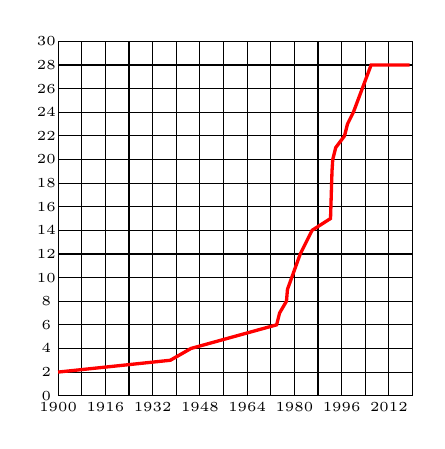
\begin{tikzpicture}[scale=0.30]%[scale=0.50, every node/.style={scale=0.1}]
	\foreach \k in {0,...,15}
		{
		\draw (\k,0) -- (\k,15);
		}
	\foreach \k in {0,...,15}
		{
		\draw (0,\k) -- (15,\k);
		}
	\node at (0,-0.5) {\tiny 1900};
	\node at (2,-0.5) {\tiny 1916};
	\node at (4,-0.5) {\tiny 1932};
	\node at (6,-0.5) {\tiny 1948};
	\node at (8,-0.5) {\tiny 1964};
	\node at (10,-0.5) {\tiny 1980};
	\node at (12,-0.5) {\tiny 1996};
	\node at (14,-0.5) {\tiny 2012};
	
	\node at (-0.5,0) {\tiny 0};
	\node at (-0.5,1) {\tiny 2};
	\node at (-0.5,2) {\tiny 4};
	\node at (-0.5,3) {\tiny 6};
	\node at (-0.5,4) {\tiny 8};
	\node at (-0.5,5) {\tiny 10};
	\node at (-0.5,6) {\tiny 12};
	\node at (-0.5,7) {\tiny 14};
	\node at (-0.5,8) {\tiny 16};
	\node at (-0.5,9) {\tiny 18};
	\node at (-0.5,10) {\tiny 20};
	\node at (-0.5,11) {\tiny 22};
	\node at (-0.5,12) {\tiny 24};
	\node at (-0.5,13) {\tiny 26};
	\node at (-0.5,14) {\tiny 28};
	\node at (-0.5,15) {\tiny 30};
	
	\draw[very thick,red] plot[samples=500] coordinates {
	(0,1)
	(4.75,1.5)
	(5.625,2)
	(9.25,3)
	(9.375,3.5)
	(9.6667,4)
	(9.7083,4.5)
	(10.25,6)
	(10.75,7)
	(11.5313,7.5)
	(11.5625,8.5)
	(11.5938,9.5)
	(11.625,10)
	(11.75,10.5)
	(12.125,11)
	(12.25,11.5)
	(12.5,12)
	(13.25,14)
	(14.875,14)
	};
	\end{tikzpicture}
	\end{figure}
\end{minipage}
\end{frame}





% Torsion Subgroup
\begin{frame}[plain]
\ctext{What about the Torsion Subgroup?}
\end{frame}





% Why Care about Torsion?
\begin{frame}[plain,fragile] \frametitle{Why Care about Torsion?}
\small
\begin{tikzcd}[scale=0.5]
	& \left\{\begin{matrix} \text{Torsion Subgroups} \\ \text{of Elliptic Curves} \end{matrix} \right\} \arrow[<->]{dl} \arrow[<->]{dr} & \\
	\left\{\begin{matrix} \text{Galois} \\ \text{Representations} \end{matrix} \right\} \arrow[<->]{rr} & & \left\{\begin{matrix} \text{Modular} \\ \text{Curves} \end{matrix} \right\}
	\end{tikzcd}
\end{frame}





%%%%%%%%%%%
% General Fields
%%%%%%%%%%%

% Boundedness: Merel, Parent
\begin{frame}[plain]
\begin{thm}[Merel, 1996; Parent, 1999]
Let $K$ be a number field of degree $d > 1$. Then
	\begin{enumerate}[(i)]
	\item (Merel) Let $E/K$ be an elliptic curve. If $E(K)$ contains a point of exact prime order $p$, then $\ell \leq d^{3d^2}$.
	\item (Parent) If $P$ is a point of exact prime power order $\ell^n$, then
		\begin{enumerate}[(a)]
		\item $\ell^n \leq 65(3^d - 1)(2d)^6$, if $\ell \geq 5$
		\item $\ell^n \leq 65(5^d - 1)(2d)^6$, if $\ell= 3$
		\item $\ell^n \leq 129(3^d - 1)(3d)^6$, if $\ell= 2$
		\end{enumerate}
	In particular, $\ell^p \leq 129(5^d - 1)(3d)^6$ for all primes $\ell$. 
	\item (Oesterl\'e) If $p \in S(d)$, then $p \leq (1 + 3^{d/2})^2$. 
	\end{enumerate}
\end{thm}
	\begin{figure}[h]
	\centering
	\begin{subfigure}{0.3\textwidth}
	\captionsetup{labelformat=empty}
	\centering
	\fbox{\includegraphics[width=0.92\textwidth]{images/merel.jpeg}}
	\caption{Lo\"ic Merel}
	\end{subfigure}
	%
	\begin{subfigure}{0.3\textwidth}
	\captionsetup{labelformat=empty}
	\centering
	\fbox{\includegraphics[width=\textwidth]{images/parent.png}}
	\caption{Pierre Parent}
	\end{subfigure} \hspace{0.05cm}
	%
	\begin{subfigure}{0.3\textwidth}
	\captionsetup{labelformat=empty}
	\centering
	\fbox{\includegraphics[width=0.92\textwidth]{images/oesterle.jpeg}}
	\caption{Joseph Oesterl\'e}
	\end{subfigure}
	\end{figure}
\end{frame}





% Q-Torsion (Mazur)
\begin{frame}[plain]
\begin{thm}[Levi-Ogg Conjecture; Mazur, 1977]
If $E/\Q$ is a rational elliptic curve, then the possible torsion subgroups $E(\Q)_\tors$ are precisely:
	\[
	\begin{cases}
	\Z/n\Z, & \text{with } n=1,2,\ldots,10,12 \text{ or} \\
	\Z/2\Z \oplus \Z/2n\Z, & \text{with } n=1,\ldots,4
	\end{cases}
	\]
Furthermore, each possibility occurs infinitely often.
\end{thm}
	\begin{figure}[h]
	\centering
	\begin{subfigure}{0.3\textwidth}
	\captionsetup{labelformat=empty}
	\centering
	\fbox{\includegraphics[width=0.72\textwidth]{images/levi.jpg}}
	\caption{Beppo Levi}
	\end{subfigure}
	%
	\begin{subfigure}{0.3\textwidth}
	\captionsetup{labelformat=empty}
	\centering
	\fbox{\includegraphics[width=\textwidth]{images/ogg.jpg}}
	\caption{Andrew Ogg}
	\end{subfigure} \hspace{0.05cm}
	%
	\begin{subfigure}{0.3\textwidth}
	\captionsetup{labelformat=empty}
	\centering
	\fbox{\includegraphics[width=0.83\textwidth]{images/mazur.jpg}}
	\caption{Barry Mazur}
	\end{subfigure}
	\end{figure}
\end{frame}





% Quadratic Number Field
\begin{frame}[plain]
\begin{thm}[Kenku, Momose, 1988; Kamienny, 1992]
 Let $K/\Q$ be a quadratic number field and $E/K$ be an elliptic curve. Then the possible torsion subgroups $E(K)_\tors$ are precisely:
 	\[
	\begin{cases}
	\Z/n\Z, & \text{with } n=1,2,\ldots,16,18 \text{ or} \\
	\Z/2\Z \oplus \Z/2n\Z, & \text{with } n=1,\ldots,6 \text{ or} \\
	\Z/3\Z \oplus \Z/3n\Z, & \text{with } n=1,2 \text{ or} \\
	\Z/4\Z \oplus \Z/4\Z
	\end{cases}
	\]
Moreover, each possibility occurs infinitely often. 
\end{thm}
	\begin{figure}[h]
	\centering
	\begin{subfigure}{0.3\textwidth}
	\captionsetup{labelformat=empty}
	\centering
	\fbox{\includegraphics[width=0.9\textwidth]{images/kenku.png}}
	\caption{Monsur Kenku}
	\end{subfigure} \;\;\;
	%
	\begin{subfigure}{0.3\textwidth}
	\captionsetup{labelformat=empty}
	\centering
	\fbox{\includegraphics[width=0.85\textwidth]{images/momose.png}}
	\caption{Fumiyuki Momose}
	\end{subfigure}
	%
	\begin{subfigure}{0.3\textwidth}
	\captionsetup{labelformat=empty}
	\centering
	\fbox{\includegraphics[width=0.63\textwidth]{images/kamienny.png}}
	\caption{Sheldon Kamienny}
	\end{subfigure}
	\end{figure}
\end{frame}





% Cubic Number Field
\begin{frame}[plain]
\small
\begin{thm}[Jeon,Kim,Schweizer, 2004; Etropolski-Morrow-Zureick Brown; Derickx, 2016]
Let $K/\Q$ be a cubic number field and $E/K$ be an elliptic curve. Then the possible torsion subgroups $E(K)_\tors$ are precisely:
	\[
	\begin{cases}
	\Z/n\Z, & \text{with } n=1,2,\ldots,16,18,20,21 \text{ or} \\
	\Z/2n\Z, & \text{with }n=1,\ldots,7
	\end{cases}
	\] 
Each of these possibilities occurs infinitely many times except for $\Z/21\Z$ which occurs only for the elliptic curve \texttt{162b1} over $\Q(\zeta_9)^+$.
\end{thm}
	\begin{figure}[h]
	\centering
	\begin{subfigure}{0.10\textwidth}
	\captionsetup{labelformat=empty}
	\centering
	\fbox{\includegraphics[width=1.2\textwidth]{images/jeon.png}}
	\caption{\hspace{0.2cm}\scriptsize{Jeon}}
	\end{subfigure} \quad\quad
	%
	\begin{subfigure}{0.10\textwidth}
	\captionsetup{labelformat=empty}
	\centering
	\fbox{\includegraphics[width=1.2\textwidth]{images/kim.jpg}}
	\caption{\hspace{0.3cm}\scriptsize{Kim}}
	\end{subfigure} \quad\quad
	%
	\begin{subfigure}{0.10\textwidth}
	\captionsetup{labelformat=empty}
	\centering
	\fbox{\includegraphics[width=1.2\textwidth]{images/schweizer.jpeg}}
	\caption{\hspace{0.1cm}\scriptsize{Schweizer}}
	\end{subfigure} \\
	%
	\hfill
	\begin{subfigure}{0.12\textwidth}
	\captionsetup{labelformat=empty}
	\centering
	\fbox{\includegraphics[width=1.7\textwidth]{images/etropolski.jpg}}
	\caption{\;\;\;\;\scriptsize{Etropolski}}
	\end{subfigure} \hspace{1.5cm}
	%
	\begin{subfigure}{0.10\textwidth}
	\captionsetup{labelformat=empty}
	\centering
	\fbox{\includegraphics[width=1.45\textwidth]{images/morrow.png}}
	\caption{\;\;\;\scriptsize{Morrow}}
	\end{subfigure} \hspace{0.6cm}
	%
	\begin{subfigure}{0.20\textwidth}
	\captionsetup{labelformat=empty}
	\centering
	\fbox{\includegraphics[width=0.55\textwidth]{images/zbrown3.jpeg}}
	\caption{\scriptsize Zureick-Brown}
	\end{subfigure} \hspace{0cm}
	%
	\begin{subfigure}{0.10\textwidth}
	\captionsetup{labelformat=empty}
	\centering
	\fbox{\includegraphics[width=1.2\textwidth]{images/derickx.jpg}}
	\caption{\;\;\scriptsize{Derickx}}
	\end{subfigure} \hfill \phantom{.}
	\end{figure}
\end{frame}





% Quartic Number Field
\begin{frame}[plain]
\begin{thm}[Jeon, Kim, Park, 2006]
Let $K/\Q$ be a quartic number field and $E/K$ be an elliptic curve. Then the possible torsion subgroups $E(K)_\tors$ appearing infinitely often are precisely:
	\[
	\begin{cases}
	\Z/n\Z, & \text{with } n=1,2,\ldots,18,20,21,22 \text{ or} \\
	\Z/2\Z \oplus \Z/2n\Z, & \text{with } n=1,\ldots,9 \text{ or} \\
	\Z/3\Z \oplus \Z/3n\Z, & \text{with } n=1,2,3 \text{ or} \\
	\Z/4\Z \oplus \Z/4n\Z, & \text{with } n=1,2 \text{ or} \\
	\Z/5\Z \oplus \Z/5\Z & \text{ or} \\
	\Z/6\Z \oplus \Z/6\Z
	\end{cases}
	\]
\end{thm}
	\begin{figure}[h]
	\centering
	\begin{subfigure}{0.3\textwidth}
	\captionsetup{labelformat=empty}
	\centering
	\fbox{\includegraphics[width=0.60\textwidth]{images/jeon.png}}
	\caption{\hspace{0.1cm}Daeyeol Jeon}
	\end{subfigure}
	%
	\begin{subfigure}{0.3\textwidth}
	\captionsetup{labelformat=empty}
	\centering
	\fbox{\includegraphics[width=0.63\textwidth]{images/kim.jpg}}
	\caption{Chang Kim}
	\end{subfigure}
	%
	\begin{subfigure}{0.3\textwidth}
	\captionsetup{labelformat=empty}
	\centering
	\fbox{\includegraphics[width=0.45\textwidth]{images/park.png}}
	\caption{\hspace{0cm}Eui-Sung Park}
	\end{subfigure}
	\end{figure}
\end{frame}



% Quintic Number Field
\begin{frame}[plain]
\begin{thm}[Derickx, Sutherland, 2016]
Let $K/\Q$ be a quintic number field and $E/K$ be an elliptic curve. Then the possible torsion subgroups $E(K)_\tors$ appearing infinitely often are precisely:
	\[
	\begin{cases}
	\Z/n\Z, & \text{with } n=1,\ldots,22,24,25 \text{ or} \\
	\Z/2\Z \oplus \Z/2n\Z, & \text{with } n=1,\ldots,8
	\end{cases}
	\]
\end{thm}
	\begin{figure}[h]
	\centering
	\begin{subfigure}{0.3\textwidth}
	\captionsetup{labelformat=empty}
	\centering
	\fbox{\includegraphics[width=0.72\textwidth]{images/derickx.jpg}}
	\caption{\hspace{0.1cm}Maarten Derickx}
	\end{subfigure}
	%
	\begin{subfigure}{0.3\textwidth}
	\captionsetup{labelformat=empty}
	\centering
	\fbox{\includegraphics[width=0.82\textwidth]{images/sutherland.jpg}}
	\caption{Drew Sutherland}
	\end{subfigure}
	\end{figure}
\end{frame}



% Sextic Number Field
\begin{frame}[plain]
\begin{thm}[Derickx, Sutherland, 2016]
Let $K/\Q$ be a sextic number field and $E/K$ be an elliptic curve. Then the possible torsion subgroups $E(K)_\tors$ appearing infinitely often are precisely:
	\[
	\begin{cases}
	\Z/n\Z, &  \text{with } n=1,\ldots,30; n \neq 23,25,29 \text{ or} \\
	\Z/2\Z \oplus \Z/2n\Z, & \text{with } n=1,\ldots,10 \text{ or} \\
	\Z/3\Z \oplus \Z/3n\Z, & \text{with } n=1,\ldots,4 \text{ or} \\
	\Z/4\Z \oplus \Z/4n\Z, & \text{with } n=1,2 \text{ or} \\
	\Z/6\Z \oplus \Z/6\Z 
	\end{cases}
	\]
\end{thm}
	\begin{figure}[h]
	\centering
	\begin{subfigure}{0.28\textwidth}
	\captionsetup{labelformat=empty}
	\centering
	\fbox{\includegraphics[width=0.72\textwidth]{images/derickx.jpg}}
	\caption{\hspace{0.1cm}Maarten Derickx}
	\end{subfigure}
	%
	\begin{subfigure}{0.28\textwidth}
	\captionsetup{labelformat=empty}
	\centering
	\fbox{\includegraphics[width=0.82\textwidth]{images/sutherland.jpg}}
	\caption{Drew Sutherland}
	\end{subfigure}
	\end{figure}
\end{frame}





%%%%%%%%%%%
% CM Curves
%%%%%%%%%%%

% CM Clark, Corn, Rice, Stankewicz
\begin{frame}[plain]
	\begin{thm}[Clark, Corn, Rice, Stankewicz; 2013]
	Let $K$ be a number field of degree $d=1,2,\ldots,13$ and $E/K$ be an elliptic curve with CM. Then all possible torsion subgroups are given, and an algorithm to compute the list.
	\end{thm} 
	\begin{figure}[h]
	\centering
	\begin{subfigure}{0.23\textwidth}
	\captionsetup{labelformat=empty}
	\centering
	\fbox{\includegraphics[width=0.75\textwidth]{images/clark.jpg}}
	\caption{Pete Clark}
	\end{subfigure}
	%
	\begin{subfigure}{0.23\textwidth}
	\captionsetup{labelformat=empty}
	\centering
	\fbox{\includegraphics[width=0.83\textwidth]{images/corn.jpg}}
	\caption{Patrick Corn}
	\end{subfigure}
	%
	\begin{subfigure}{0.23\textwidth}
	\captionsetup{labelformat=empty}
	\centering
	\fbox{\includegraphics[width=1.0\textwidth]{images/rice.png}}
	\caption{Alex Rice}
	\end{subfigure}
	%
	\begin{subfigure}{0.25\textwidth}
	\captionsetup{labelformat=empty}
	\centering
	\fbox{\includegraphics[width=0.65\textwidth]{images/stankewicz.png}}
	\caption{James Stankewicz}
	\end{subfigure}
	\end{figure}
\end{frame}




% CM Bourdon Clark Stankewicz
\begin{frame}[plain]
\footnotesize
\begin{thm}[Bourdon, Clark, Stankewicz, 2015]
Let $F$ be a number field of odd degree, let $E/F$ be a $K$-CM elliptic curve, and let $T= E(F)_\tors$. Then
	\begin{enumerate}[(a)]
	\item One of the following occurs:
		\begin{enumerate}[(i)] \footnotesize
		\item $T$ is isomorphic to the trivial group $\O$, $\Z/2\Z$, $\Z/4\Z$, or $\Z/2\Z \times \Z/2\Z$;
		\item $T \cong \Z/\ell^n\Z$ for a prime $\ell \equiv 3 \mod 8$ and $n \in \Z^+$ and $K= \Q(\sqrt{-\ell})$;
		\item $T \cong \Z/2\ell^n\Z$ for a prime $\ell \equiv 3 \mod 4$ and $n \in \Z^+$ and $K= \Q(\sqrt{-\ell})$. 
		\end{enumerate}
	\item If $E(F)_\tors \cong \Z/2\Z \oplus \Z/2\Z$, then $\End E$ has discriminant $\Delta= -4$.
	\item If $E(F)_\tors \cong \Z/4\Z$, then $\End E$ has discriminant $\Delta \in \{ -4, -16 \}$.
	\item Each of the groups listed in part (a) arises up to isomorphism as the torsion subgroup $E(F)$ of a CM elliptic curve $E$ defined over an odd degree number field $F$. 
	\end{enumerate}
\end{thm}
	\begin{figure}[h]
	\centering
	\begin{subfigure}{0.30\textwidth}
	\captionsetup{labelformat=empty}
	\centering
	\fbox{\includegraphics[width=0.65\textwidth]{images/bourdon.png}}
	\caption{\scriptsize Abbey Bourdon}
	\end{subfigure}
	%
	\begin{subfigure}{0.30\textwidth}
	\captionsetup{labelformat=empty}
	\centering
	\fbox{\includegraphics[width=0.56\textwidth]{images/clark.jpg}}
	\caption{\scriptsize Pete Clark}
	\end{subfigure}
	%
	\begin{subfigure}{0.30\textwidth}
	\captionsetup{labelformat=empty}
	\centering
	\fbox{\includegraphics[width=0.53\textwidth]{images/stankewicz.png}}
	\caption{\scriptsize James Stankewicz}
	\end{subfigure}
	\end{figure}
\end{frame}





% CM Bourdon Pollack
\begin{frame}[plain]
	\begin{thm}[Bourdon, Pollack; 2018]
	Let $K$ be an odd degree number field and $E/K$ be an elliptic curve with CM. Then the torsion subgroups $E(K)_\tors$ are computable. 
	\end{thm} 
	\begin{figure}[h]
	\centering
	\begin{subfigure}{0.3\textwidth}
	\captionsetup{labelformat=empty}
	\centering
	\fbox{\includegraphics[width=0.85\textwidth]{images/bourdon.png}}
	\caption{Abbey Bourdon}
	\end{subfigure}
	%
	\begin{subfigure}{0.3\textwidth}
	\captionsetup{labelformat=empty}
	\centering
	\fbox{\includegraphics[width=0.82\textwidth]{images/pollack.jpg}}
	\caption{Paul Pollack}
	\end{subfigure}
	\end{figure}
\end{frame}



%%%%%%%%%%%
% Rational Elliptic 
%%%%%%%%%%%

% Quadratic Rational EC
\begin{frame}[plain]
\footnotesize
\begin{thm}[Najman, 2015]
Let $E/\Q$ be a rational elliptic curve, and let $K/\Q$ be a quadratic number field. Then the possible torsion subgroups $E(K)_\tors$ are precisely:
	\[
	\begin{cases}
	\Z/n\Z, & \text{with } n= 1, 2, \ldots, 10, 12, 15, 16 \text{ or} \\
	\Z/2\Z \oplus \Z/2n\Z, & \text{with } n= 1, 2, \ldots, 6 \text{ or} \\
	\Z/3\Z \oplus \Z/3n\Z, & \text{with } n= 1, 2 \text{ or} \\
	\Z/4\Z \oplus \Z/4\Z
	\end{cases}
	\]
Each such possibility occurs for infinitely many elliptic curves except for $\Z/15\Z$, which occurs only for the elliptic curves \texttt{50b1} and \texttt{50a3} over $\Q(\sqrt{5})$ and the elliptic curves \texttt{50b2} and \texttt{450b4} over $\Q(\sqrt{-15})$. 
\end{thm}
	\begin{figure}[!ht]
	\centering
	\captionsetup{labelformat=empty}
	\fbox{\includegraphics[width=0.18\textwidth]{images/najman2.png}}
	\caption{Filip Najman}
	\end{figure}
\end{frame}





% Cubic Rational EC
\begin{frame}[plain]
\begin{thm}[Najman, 2015]
Let $E/\Q$ be a rational elliptic curve, and let $K/\Q$ be a cubic number field. Then the possible torsion subgroups $E(K)_\tors$ are precisely:
	\[
	\begin{cases}
	\Z/n\Z, & \text{with } n= 1, 2, \ldots, 10, 12, 13, 14, 18, 21 \text{ or} \\
	\Z/2\Z \oplus \Z/2n\Z, & \text{with } n= 1, 2, 3, 4, 7
	\end{cases}
	\]
Each such possibility occurs for infinitely many elliptic curves except for $\Z/21\Z$, which only occurs for the elliptic curve \texttt{162b1} over $\Q(\zeta_9)^+$.
\end{thm}
	\begin{figure}[!ht]
	\centering
	\captionsetup{labelformat=empty}
	\fbox{\includegraphics[width=0.18\textwidth]{images/najman2.png}}
	\caption{Filip Najman}
	\end{figure}
\end{frame}





% Quartic Rational EC
\begin{frame}[plain]
\footnotesize
\begin{thm}[Chou, 2015; Gonz\'alez-Jimenez, Lozano-Robledo, 2016; Gonz\'alez-Jimenez, Najman, 2016]
Let $E/\Q$ be a rational elliptic curve, and let $K/\Q$ be a quartic number field. Then the possible torsion subgroups $E(K)_\tors$ are precisely:
	\[
	\begin{cases}
	\Z/n\Z, & \text{with } n= 1, 2, \ldots, 10, 12, 13, 15, 16, 20, 24 \text{ or} \\
	\Z/2\Z \oplus \Z/2n\Z, & \text{with } n= 1, 2, \ldots, 6, 8 \text{ or} \\
	\Z/3\Z \oplus \Z/3n\Z, & \text{with } n= 1, 2 \text{ or} \\
	\Z/4\Z \oplus \Z/4n\Z, & \text{with } n= 1, 2 \text{ or} \\
	\Z/5\Z \oplus \Z/5\Z, & \text{or} \\
	\Z/6\Z \oplus \Z/6\Z 
	\end{cases}
	\]
Each such possibility occurs for infinitely many elliptic curves except for $\Z/15\Z$, which occurs only for the elliptic curves with $j(E) \in \{ -5^2/2, -5^2 \cdot 241^3/2^3$, $-5 \cdot 29^3/2^5, 5 \cdot 211^3/2^{15} \}$ over some quartic field. 
\end{thm}
	\begin{figure}[h]
	\centering
	\begin{subfigure}{0.20\textwidth}
	\captionsetup{labelformat=empty}
	\centering
	\fbox{\includegraphics[width=0.66\textwidth]{images/chou.jpg}}
	\caption{\tiny Michael Chou}
	\end{subfigure} \quad
	%
	\begin{subfigure}{0.20\textwidth}
	\captionsetup{labelformat=empty}
	\centering
	\fbox{\includegraphics[width=0.51\textwidth]{images/jimenez2.jpeg}}
	\caption{\tiny \hspace{0.7cm}Enrique \\ \;\;\;Gonz\'alez-Jim\'enez}
	\end{subfigure}
	%
	\begin{subfigure}{0.20\textwidth}
	\captionsetup{labelformat=empty}
	\centering
	\fbox{\includegraphics[width=0.76\textwidth]{images/robledo.jpg}}
	\caption{\tiny \hspace{0.7cm}\'Alvaro \\ \;\;\;\;\;Lozano-Robledo}
	\end{subfigure} \quad
	%
	\begin{subfigure}{0.20\textwidth}
	\captionsetup{labelformat=empty}
	\centering
	\fbox{\includegraphics[width=0.58\textwidth]{images/najman2.png}}
	\caption{\tiny Filip Najman}
	\end{subfigure}
	\end{figure}
\end{frame}





% Quintic Rational EC
\begin{frame}[plain]
\begin{thm}[Gonz\'alez-Jimenez, 2016]
Let $E/\Q$ be a rational elliptic curve, and let $K/\Q$ be a quintic number field. Then the possible torsion subgroups $E(K)_\tors$ are precisely:
	\[
	\begin{cases}
	\Z/n\Z, & \text{with } n= 1, 2, \ldots, 12, 25 \text{ or} \\
	\Z/2\Z \oplus \Z/2n\Z, & \text{with } n= 1, 2, 3, 4
	\end{cases}
	\]
Each of these possibilities occurs infinitely many times except for $\Z/11\Z$ which occurs for the elliptic curves \texttt{121a2}, \texttt{121c2}, and \texttt{121b1} over some quintic field. 
\end{thm}
	\begin{figure}[!ht]
	\centering
	\captionsetup{labelformat=empty}
	\fbox{\includegraphics[width=0.18\textwidth]{images/jimenez2.jpeg}}
	\caption{Enrique Gonz\'alez-Jim\'enez}
	\end{figure}
\end{frame}





% Sextic Rational EC
\begin{frame}[plain]
\footnotesize
\begin{thm}[Daniels, Gonz\'alez-Jimenez, 2018; Gu{\u{z}}vi\'c, 2019]
Let $E/\Q$ be a rational elliptic curve, and let $K/\Q$ be a sextic number field. Then the possible torsion subgroups $E(K)_\tors$ are among:
	\[
	\begin{cases}
	\Z/n\Z, & \text{with } n= 1, 2, \ldots, 16, 18, 21, 30, n \neq 11  \text{ or} \\
	\Z/2\Z \oplus \Z/2n\Z, & \text{with } n= 1, 2, \ldots, 7, 9 \text{ or} \\
	\Z/3\Z \oplus \Z/3n\Z, & \text{with } n= 1, 2, 3, 4, 6^* \text{ or} \\
	\Z/4\Z \oplus \Z/4n\Z, & \text{with } n= 1, 3 \\
	\Z/6\Z \oplus \Z/6\Z 
	\end{cases}
	\]
Each such possibility occurs for infinitely many elliptic curves except for $\Z/15\Z$, $\Z/21\Z$, $\Z/30\Z$, $\Z/4\Z \oplus \Z/12\Z$, and possibly $\Z/3\Z \oplus \Z/18\Z$. 
\end{thm}
	\begin{figure}[h]
	\centering
	\begin{subfigure}{0.30\textwidth}
	\captionsetup{labelformat=empty}
	\centering
	\fbox{\includegraphics[width=0.65\textwidth]{images/daniels.jpeg}}
	\caption{\tiny Harris Daniels}
	\end{subfigure} 
	%
	\begin{subfigure}{0.30\textwidth}
	\captionsetup{labelformat=empty}
	\centering
	\fbox{\includegraphics[width=0.42\textwidth]{images/jimenez2.jpeg}}
	\caption{\tiny \hspace{0.4cm} Enrique Gonz\'alez-Jim\'enez}
	\end{subfigure}
	%
	\begin{subfigure}{0.30\textwidth}
	\captionsetup{labelformat=empty}
	\centering
	\fbox{\includegraphics[width=0.90\textwidth]{images/guzvic.png}}
	\caption{\tiny Tomislav Gu{\u{z}}vi\'c}
	\end{subfigure}
	\end{figure}
\end{frame}





% Other Fields Rational EC
\begin{frame}[plain]
\begin{thm}[Gonz\'alez-Jimenez, Najman, 2016]
Let $E/\Q$ be a rational elliptic curve, and let $K/\Q$ be a number field whose smallest prime divisor is at least 7, then the only possible torsion subgroups $E(\Q)_\tors$ are those from Mazur's list, namely:
	\[
	\begin{cases}
	\Z/n\Z, & \text{with } n= 1, 2, \ldots, 10, 12 \text{ or} \\
	\Z/2\Z \oplus \Z/2n\Z, & \text{with } n= 1, 2, 3, 4
	\end{cases}
	\]
Each such possibility occurs for infinitely many elliptic curves. In fact, if the largest prime divisor is at least 11, then $E(K)_\tors=$ $E(\Q)_\tors$. 
\end{thm}
	\begin{figure}[h]
	\centering
	\begin{subfigure}{0.40\textwidth}
	\captionsetup{labelformat=empty}
	\centering
	\fbox{\includegraphics[width=0.40\textwidth]{images/jimenez2.jpeg}}
	\caption{\footnotesize \hspace{0.4cm} Enrique Gonz\'alez-Jim\'enez}
	\end{subfigure}
	%
	\begin{subfigure}{0.40\textwidth}
	\captionsetup{labelformat=empty}
	\centering
	\fbox{\includegraphics[width=0.45\textwidth]{images/najman2.png}}
	\caption{\footnotesize Filip Najman}
	\end{subfigure}
	\end{figure}
\end{frame}





% Quartic Galois Rational EC
\begin{frame}[plain]
\small
\begin{thm}[Chou, 2015]
Let $E/\Q$ be a rational elliptic curve, and let $K/\Q$ be a quartic Galois number field. Then the possible torsion subgroups $E(K)_\tors$ are precisely:
	\[
	\begin{cases}
	\Z/n\Z, & \text{with } n= 1, 2, \ldots, 10, 12, 13, 15, 16 \text{ or} \\
	\Z/2\Z \oplus \Z/2n\Z, & \text{with } n= 1, 2, \ldots, 6, 8 \text{ or} \\
	\Z/3\Z \oplus \Z/3n\Z, & \text{with } n= 1, 2 \text{ or} \\
	\Z/4\Z \oplus \Z/4n\Z, & \text{with } n= 1, 2 \text{ or} \\
	\Z/5\Z \oplus \Z/5\Z, & \text{or} \\
	\Z/6\Z \oplus \Z/6\Z 
	\end{cases}
	\]
\end{thm}
	\begin{figure}[!ht]
	\centering
	\captionsetup{labelformat=empty}
	\fbox{\includegraphics[width=0.20\textwidth]{images/chou.jpg}}
	\caption{Michael Chou}
	\end{figure}
\end{frame}




%%%%%%%%%%%
% Infinite Extensions 
%%%%%%%%%%%

% Maximal 2-Abelian
\begin{frame}[plain]
\footnotesize
\begin{thm}[Laska, Lorenz, 1985; Fujita, 2005]
Let $E/\Q$ be a rational elliptic curve, and let $\Q(2^\infty)$ be the maximal abelian 2-extension of $\Q$. Then $E(K)_\tors$ is isomorphic to precisely one of the following groups:
	\[
	\begin{cases}
	\Z/n\Z, & \text{with } n= 1, 3, 5, 7, 9, 15 \text{ or} \\
	\Z/2\Z \oplus \Z/2n\Z, & \text{with } n= 1, 2, 3, 4, 5, 6, 8 \text{ or} \\
	\Z/3\Z \oplus \Z/3\Z, & \text{ or} \\
	\Z/4\Z \oplus \Z/4n\Z, & \text{with } n= 1, 2, 3, 4 \text{ or} \\
	\Z/2n\Z \oplus \Z/2n\Z, & \text{with } n= 3, 4
	\end{cases}
	\]
and each such possibility occurs. 
\end{thm}
	\begin{figure}[h]
	\centering
	\begin{subfigure}{0.30\textwidth}
	\captionsetup{labelformat=empty}
	\centering
	\fbox{\includegraphics[width=0.42\textwidth]{images/laska.png}}
	\caption{\scriptsize Michael Laska}
	\end{subfigure}
	%
	\begin{subfigure}{0.30\textwidth}
	\captionsetup{labelformat=empty}
	\centering
	\fbox{\includegraphics[width=0.46\textwidth]{images/lorenz.jpeg}}
	\caption{\scriptsize Martin Lorenz}
	\end{subfigure}
	%
	\begin{subfigure}{0.30\textwidth}
	\captionsetup{labelformat=empty}
	\centering
	\fbox{\includegraphics[width=0.47\textwidth]{images/fujita.png}}
	\caption{\scriptsize Yasutsugu Fujita}
	\end{subfigure}
	\end{figure}
\end{frame}





% Maximal 3-Abelian
\begin{frame}[plain]
\footnotesize
\begin{thm}[Daniels, Lozano-Robledo, Najman, Sutherland, 2017]
Let $E/\Q$ be a rational elliptic curve. Then the torsion subgroup $E(\Q(3^\infty))_\tors$ is finite and is isomorphic to precisely one of the following groups:
	\[
	\begin{cases}
	\Z/2\Z \oplus \Z/2n\Z, & \text{with } n= 1, 2, 4, 5, 7, 8, 13 \text{ or} \\
	\Z/4\Z \oplus \Z/4n\Z, & \text{with } n= 1, 2, 4, 7 \text{ or} \\
	\Z/6\Z \oplus \Z/6n\Z, & \text{with } n= 1, 2, 3, 5, 7 \text{ or} \\
	\Z/2n\Z \oplus \Z/2n\Z, & \text{with } n= 4, 6, 7, 9 \\
	\end{cases}
	\]
All but four of the torsion subgroups, $T$, listed above occur for infinitely many $\ov{\Q}$-isomorphism classes of elliptic curves $E/\Q$. For $T \cong \Z/4\Z \oplus \Z/28\Z$, $\Z/6\Z \oplus \Z/30\Z$, $\Z/6\Z \oplus \Z/42\Z$, and $\Z/14\Z \oplus \Z/14\Z$, there are only 2, 2, 4, and 1 (respectively) $\ov{\Q}$-isomorphism classes of $E/\Q$ for which $E(\Q(3^\infty))_\tors \cong T$. 
\end{thm}
	\begin{figure}[h]
	\centering
	\begin{subfigure}{0.23\textwidth}
	\captionsetup{labelformat=empty}
	\centering
	\fbox{\includegraphics[width=0.85\textwidth]{images/daniels.jpeg}}
	\caption{\scriptsize Harris Daniels}
	\end{subfigure}
	%
	\begin{subfigure}{0.23\textwidth}
	\captionsetup{labelformat=empty}
	\centering
	\fbox{\includegraphics[width=0.75\textwidth]{images/lozano.jpeg}}
	\caption{\scriptsize \hspace{0.70cm}\'Alvaro \\ \;\;Lozano-Robledo}
	\end{subfigure}
	%
	\begin{subfigure}{0.23\textwidth}
	\captionsetup{labelformat=empty}
	\centering
	\fbox{\includegraphics[width=0.60\textwidth]{images/najman2.png}}
	\caption{\scriptsize Filip Najman}
	\end{subfigure}
	%
	\begin{subfigure}{0.23\textwidth}
	\captionsetup{labelformat=empty}
	\centering
	\fbox{\includegraphics[width=0.77\textwidth]{images/sutherland.jpg}}
	\caption{\scriptsize Andrew Sutherland}
	\end{subfigure}
	\end{figure}
\end{frame}





% Maximal Abelian Extension
\begin{frame}[plain]
\footnotesize
\begin{thm}[Chou, 2019]
Let $E/\Q$ be a rational elliptic curve. Then $E(\Q^{\text{ab}})_\tors$ is finite, and is isomorphic to precisely one of the following groups:
	\[
	\begin{cases}
	\Z/n\Z, & n= 1, 3, 5, 7, 9, 11, 13, 15, 17, 19, 21, 25, 27, 37, 43, 67, 163 \\
	\Z/2\Z \oplus \Z/2n\Z, & n= 1, 2, \ldots, 9 \\
	\Z3\Z \oplus \Z/3n\Z, & n= 1, 3 \\
	\Z/4\Z \oplus \Z/4n\Z, & n= 1, 2, 3, 4 \\
	\Z/n\Z \oplus \Z/n\Z, & n= 5, 6, 8
	\end{cases}
	\]
Each of the listed groups appears as a torsion subgroup for $E(\Q^{\text{ab}})_\tors$ for some elliptic curve over $\Q$. 
\end{thm}
	\begin{figure}[!ht]
	\centering
	\captionsetup{labelformat=empty}
	\fbox{\includegraphics[width=0.20\textwidth]{images/chou.jpg}}
	\caption{Michael Chou}
	\end{figure}
\end{frame}





%%%%%%%%%%%
% Technical Pieces
%%%%%%%%%%%

% Technical Preliminaries
\begin{frame}[plain]
\ctext{Technical Preliminaries}
\end{frame}





%
\begin{frame}[plain] \frametitle{$j$-invariant \& Twists}
\footnotesize
	\[
	y^2 + a_1xy + a_3y= x^3 + a_2x^2 + a_4x + a_6.
	\] \pspace
Define $b_2= a_1^2 + 4a_2$, $b_4= 2a_4 + a_1a_3$, and $b_6= a_3^2 + 4a_5$.
	\[
	\begin{aligned}
	b_8&= a_1^2a_6 + 4a_2a_6 - a_1a_3a_4 + a_2a_3^2 - a_4^2 &\quad&& \Delta_E&= -b_2^2b_8 - 8b_4^3 - 27b_6^2 + 9b_2b_4b_6 \\
	c_4&= b_2^2 - 24b_4 &&& c_6&= -b_2^3 + 36b_2b_4 - 216b_6
	\end{aligned}
	\]
Then the $j$-invariant of $E$ is\dots
	\[
	 j= \dfrac{c_4^3}{\Delta_E}
	\]
Furthermore, if $E: y^2= x^3 + Ax + B$, then a (quadratic) twist of $E$ by $d \in K$ squarefree, denoted $E^{(d)}$, is
	\[
	E^{(d)}: dy^2= x^3 + Ax + B \cong E^{(d)}: y^2= x^3 + d^2Ax + d^3B 
	\]
The elliptic curves $E$ and $E^{(d)}$ have the same $j$-invariant, namely $j= -1728 \,\dfrac{(4A)^3}{\Delta}$. An elliptic curve with $j$-invariant $j_0$ is\dots
	\[
	E \colon y^2 + xy= x^3 - \dfrac{36}{j_0 - 1728}\,x - \dfrac{1}{j_0 - 1728}.
	\]
\end{frame}





% Division Polynomials
\begin{frame}[plain] \frametitle{Division Polynomials}
\footnotesize
Given an elliptic curve $E: y^2= x^3 + Ax + B$, define\dots
	\[
	\psi_{E,n}= 
	\begin{cases}
	1, & \text{for } n= 1, \\
	2y, & \text{for } n= 2, \\
	3x^4 + 6Ax^2 + 12Bx - A^2, & \text{for } n= 3, \\
	4y(x^6 + 5Ax^4 + 20Bx^3 - 5A^2x^2 - 4ABx - 8B^2 - A^3), & \text{for } n= 4.
	\end{cases}
	\]
We define $\psi_n$ for $n > 4$ using the recursive relations 
	\[
	\begin{cases}
	\psi_{E,{2n+1}}= \psi_{n+2} \psi_n^3 - \psi_{n-1} \psi_{n+1}^3, & \text{if } n \geq 2 \\
	2y\psi_{E,2n}= \psi_m (\psi_{n+2} \psi_{n-1}^2 - \psi_{n-2} \psi_{n+1}^2), & \text{if } n \geq 3.
	\end{cases}
	\]
For some polynomials $\phi_n(x)$ and $\omega_n(x,y)$, we have
	\[
	[n]P= \left( \dfrac{\phi_n(x)}{\psi_{E,n}^2(x)}, \dfrac{\omega_n(x,y)}{\psi_{E,n}(x,y)^2} \right). 
	\]

{\itshape Note: Twisting changes the division polynomial only by a rational multiple.}
\end{frame}





% Division Polynomial Method
\begin{frame}[plain] \frametitle{Division Polynomial Method}
Let $E/\Q$ be a rational elliptic curve given by $y^2= x^3 + Ax + B$, and let $P= (x,y) \in E(\ov{Q})$ be a point of order $n$. If $n$ is odd, then the $x$-coordinate of $P$ is a root of $\psi_{E,n}$. If $n$ is even, the $x$-coordinate of $P \in E[n] \setminus E[2]$ are the roots of $\psi_{E,n}/\psi_{E,2}$. \pspace

Let $f_{E,n}$ denote the primitive $n$-division polynomial associated to $\psi_{E,2}$, i.e. a polynomial whose roots are the $x$-coordinates of points $P \in E[n]$ of exact order $n$. The $y$-coordinate is then defined over at most a quadratic extension. \pspace

Note that if $p$ is prime, then $\psi_{E,n}= f_{E,n}$. For composite $n$, we have
	\[
	f_{E,n}= \dfrac{\psi_{E,n}}{\prod_{\substack{d \mid n \\ d \neq n}} f_{E,d}}.
	\]
\end{frame}





% Galois Representations
\begin{frame}[plain] \frametitle{Galois Representations}
\footnotesize
Let $E/\Q$ be a rational elliptic curve, and fix an integer $n \geq 2$. The absolute Galois group $G_\Q:= \Gal(\ov{\Q}/\Q)$ acts coordinate-wise on the points of $E[n]$. We then obtain a representation
	\[
	\rho_{E,n} \colon \Gal(\ov{\Q}/\Q) \to \Aut(E[n]).
	\]
But $E[n]$ is a free rank two $\Z/n\Z$-module. Fixing a basis, say $\{ P, Q \}$, for $E[n]$, we know that $\Aut(E[n])$ is isomorphic to a subgroup of $\GL_2(\Z/n\Z)$. We then have a map
	\[
	\rho_{E,n} \colon \Gal(\ov{\Q}/\Q) \ma{} \Aut(E[n]) \ma{} \GL_2(\Z/n\Z).
	\]
Denote by $G_E(n)$ the image of $\rho_{E,n}$ under this composition. While the exact image of this composition depends on the choice of basis, it is unique up to conjugacy. 

\begin{itemize}
\item $\ker \rho_{E,n}= \Gal(\ov{\Q}/\Q(E[n]))$
\item $G_E(n) \cong \Gal(\Q(E[n])/\Q)$
\item Let $H$ be the subgroup of $\Gal(\Q(E[n])/\Q)$ corresponding to $\Q(E[n])^H= \Q(P)$, i.e. $\Q(P)$ is the subfield of $\Q(E[n])$ fixed by $H$. 
\item Define $\widetilde{H}:= \rho_{E,n}(H)$. We then have $[\Q(P) \colon \Q]= |G_E(n) \colon \widetilde{H}|$. 
\end{itemize}
\end{frame}





%%%%%%%%%%%
% Nonic Galois Classification
%%%%%%%%%%%

% Nonic Galois Classification
\begin{frame}[plain]
\ctext{Nonic Galois Classification}
\end{frame}



% Outline
\begin{frame}[plain]
\frametitle{Outline of the Classification}
        \begin{enumerate}
        \item Determine the possible prime orders. \vfill
        \item Bound the $p$-Sylow Subgroups. \vfill
        \item Create a finite list of possibilities. \vfill
        \item Find examples and eliminate cases. \vfill
        \end{enumerate}
\vfill
\end{frame}





% Step 1. Determine the Possible Prime Orders
\begin{frame}[plain]
\vfill
\begin{center} {\bfseries \Large \textcolor{UniGray}{Step 1. Determine the Possible Prime Orders}} \end{center}
\vfill 
\end{frame}





% Lozano-Robledo S(d)
\begin{frame}[plain]
\begin{thm}[Lozano-Robledo, 2013]
Let $S_\Q(d)$ be the set of primes such that there exists an elliptic curve $E/\Q$ with a point of order $p$ defined in an extension $K/\Q$ of degree at most $d$. Then $S_\Q(9)= \{ 2, 3, 5, 7, 11, 13, 17, 19 \}$.
\end{thm}
	\begin{figure}[h]
	\centering
	\begin{subfigure}{\textwidth}
	\captionsetup{labelformat=empty}
	\centering
	\fbox{\includegraphics[width=0.2\textwidth]{images/robledo.jpg}}
	\caption{\'Alvaro Lozano-Robledo}
	\end{subfigure}
	\end{figure}

\begin{rem}
Lozano-Robledo computes $S_\Q(d)$ for $1 \leq d \leq 21$ and gives a conjectural formula for $d \geq 1$, which is valid for $1 \leq d \leq 42$, which would follow from a positive answer to Serre's uniformity question. 
\end{rem}
\end{frame}





% Gonzalez-Jimenez, Najman R(d)
\begin{frame}[plain]
\begin{prop}[Gonz\'alez-Jim\'enez, Najman, 2016] \hfill
	\begin{enumerate}[(i)]
	\item $11 \in R_\Q(d)$ if and only if $5 \mid d$.
	\item $17 \in R_\Q(d)$ if and only if $8 \mid d$.
	\end{enumerate}
\end{prop}
	\begin{figure}[h]
	\centering
	\begin{subfigure}{0.35\textwidth}
	\captionsetup{labelformat=empty}
	\centering
	\fbox{\includegraphics[width=0.65\textwidth]{images/jimenez.png}}
	\caption{Enrique Gonz\'alez-Jim\'enez}
	\end{subfigure}
	%
	\begin{subfigure}{0.3\textwidth}
	\captionsetup{labelformat=empty}
	\centering
	\fbox{\includegraphics[width=0.70\textwidth]{images/najman2.png}}
	\caption{Filip Najman}
	\end{subfigure}
	\end{figure}
\end{frame}





% Prime Possible
\begin{frame}[plain]
\begin{prop}
Let $E/\Q$ be a rational elliptic curve, and let $K/\Q$ be a nonic Galois field. If $P \in E(K)$ is a point of prime order $p$, then $p \in \{ 2, 3, 5, 7, 13,$ $19 \}$.
\end{prop}
\end{frame}





% Step 2. Bound the Size of the Sylow Subgroups
\begin{frame}[plain]
\vfill
\begin{center} {\bfseries \Large \textcolor{UniGray}{Step 2. Bound the Size of the Sylow Subgroups}} \end{center}
\vfill 
\end{frame}





% Rouse, Zureick-Brown, 2-adic
\begin{frame}[plain]
\begin{thm}[Rouse, Zureick-Brown, 2015]
Let $E/\Q$ be a rational elliptic curve without CM. Then the index of $\rho_{E,2^\infty}(\Gal(\overline{\Q}/\Q))$ divides 64 or 96, and all such indices occur. Furthermore, the image of $\rho_{E,2^\infty}(\Gal(\overline{\Q}/\Q))$ is the inverse image in $\GL_2(\Z_2)$ of the image of $\rho_{E,32}(\Gal(\overline{\Q}/\Q))$.
\end{thm}
	\begin{figure}[h]
	\centering
	\begin{subfigure}{0.3\textwidth}
	\captionsetup{labelformat=empty}
	\centering
	\fbox{\includegraphics[width=0.70\textwidth]{images/rouse.jpg}}
	\caption{Jeremy Rouse}
	\end{subfigure}
	%
	\begin{subfigure}{0.3\textwidth}
	\captionsetup{labelformat=empty}
	\centering
	\fbox{\includegraphics[width=0.69\textwidth]{images/zbrown.png}}
	\caption{David Zureick-Brown}
	\end{subfigure}
	\end{figure}
\begin{rem}
They also enumerate all 1,208 possibilities and find their rational points. 
\end{rem}
\end{frame}



% Full 2-Torsion, Lozano-Robledo
\begin{frame}[plain]
\begin{thm}[Gonz\'alez-Jim\'enez, Lozano-Robledo]
Let $E/\Q$ be an elliptic curve without CM. Let $1 \leq s \leq N$ be fixed integers, and let $T \subseteq E[2^N]$ be a subgroup isomorphic to $\Z/2^s/Z \oplus \Z/2^N \Z$. Then $[\Q(T) \colon \Q]$ is divisible by 2 if $s=N=2$, and otherwise by $2^{2N+2s-8}$ if $N \geq 3$, unless $s \geq 4$ and $j(E)$ is one of the two values:
	\[
	- \dfrac{3 \cdot 18249920^3}{17^{16}}\; \text{ or } - \dfrac{7 \cdot 1723187806080^3}{79^{16}}
	\]
in which case $[\Q(T) \colon \Q]$ is divisible by $3 \cdot 2^{2N+2s-9}$. Moreover, this is best possible in that there are one-parameter families $E_{s,N}(t)$ of elliptic curves over $\Q$ such that for each $s, N \geq 0$ and each $t \in \Q$, and subgroups $T_{s,N} \in E_{s,N}(t)(\ov{\Q})$ isomorphic to $\Z/2^s\Z \oplus \Z/2^N\Z$ such that $[\Q(T_{s,N}) \colon \Q]$ is equal to the bound given above. 
\end{thm}
\end{frame}



% 2-Sylow Bound
\begin{frame}[plain,t] 
\begin{lem}[2-Sylow Bound]
Let $E/\Q$ be a rational elliptic curve, and let $K/\Q$ be a nonic Galois field. Then $E(K)[2^\infty] \subseteq \Z/2\Z \oplus \Z/8\Z$.
\end{lem}

\pf 
\begin{itemize}
\item {\itshape $E$ has CM}: 
	\begin{enumerate}[--]
	\item From Bourdon, Clark, Stankewicz, we know that $E(K)[2^\infty] \in \{ \O, \Z/2\Z, \Z/4\Z, \Z/2\Z \oplus \Z/2\Z \}$. 
	\end{enumerate} \pspace

\item {\itshape $E$ does not have CM}: $\Z/2^s\Z \oplus \Z/2^N\Z$
	\begin{enumerate}[--]
	\item Lozano-Robledo's result (valid for $1 \leq s \leq N$) with $s= 1$, $N= 4$ and $s= N= 2$, we would have $2 \mid d= [K \colon \Q]$, a contradiction. Therefore, $E(K)[2^\infty] \not\supseteq \Z/2\Z \oplus \Z/16\Z$ or $\Z/4\Z \oplus \Z/4\Z$. \pspace
	
	Only case to consider is when $s= 0$, $N \geq 0$. We will show $E(K)[2^\infty] \not\supseteq \Z/16\Z$. 
	\end{enumerate}
\end{itemize}
\end{frame}





% 2-Sylow Bound
\begin{frame}[plain,t] 
\footnotesize
\begin{lem}[Najman, 2015]
If $E(\Q)$ has a nontrivial 2-Sylow subgroup, then $E(K)[2^\infty]= E(\Q)[2^\infty]$. 
\end{lem}

\begin{enumerate}[--]
\item Suppose $E(K)[2^\infty] \supseteq \Z/16\Z$. 
	\begin{enumerate}[(i)] \footnotesize
	\item {\itshape Rational 2-torsion}: If $E(\Q)[2^\infty] \neq \{ \O \}$, then $E(K)[2^\infty]= E(\Q)[2^\infty] \supseteq \Z/16\Z$ by Najman's Lemma, contradicting Mazur's classification of $\Phi(1)$. \pspace
	\item {\itshape No Rational 2-torsion}: Choosing a model $E: y^2= x^3 + Ax + B$, a point of order 2 is a root of $x^3 + Ax + B$, now necessarily defined over a cubic field. We know that a cubic subfield of $K$ is Galois. But then it is a splitting field so that $E(K)[2^\infty] \supseteq \Z/2\Z \oplus \Z/2\Z$, a contradiction. \hfill \qed
	\end{enumerate}
\end{enumerate}

\begin{rem} 
A general result by Gu{\u{z}}vi\'c for elliptic curves with $j(E) \in \Q$ over odd degree fields, $E(K)_\tors \not\supseteq \Z/16\Z$, which gives the same bound. Furthermore, we shall see that for elliptic curves over odd degree Galois fields, we always have $E(K)[2^\infty]= E(F)[2^\infty]$ for some cubic number field $F$. The classification of $\Phi_\Q(3)$ then gives the same bound. 
\end{rem}
\end{frame}





% Full p-Torsion & Weil-Pairing
\begin{frame}[plain]
\footnotesize
\begin{lem}[Odd Torsion]
Let $K/\Q$ be an odd degree number field, and let $E/\Q$ be a rational elliptic curve. Then $E(K)_\tors$ does not contain full $p$-torsion for all odd primes.
\end{lem}

\pf By the existence of the Weil-pairing, if $E(K)$ contains full $p$-torsion, then $\Q(\zeta_p) \subseteq K$. But for $p > 2$, $[\Q(\zeta_p) \colon \Q]= \phi(p)$ is even, a contradiction. \hfill \qed \vfill

\begin{lem}[Galois Isogeny]
Let $K/\Q$ be a Galois extension, and let $E/\Q$ be a rational elliptic curve. If $E(K)[n] \cong \Z/n\Z$, then $E$ has a rational $n$-isogeny. 
\end{lem}

\pf Let $\{ P, Q \}$ be a basis for $E[n]$. Without loss of generality, assume $P \in E(K)$ and $Q \notin E(K)$. Let $\sigma \in \Gal(\ov{\Q}/\Q)$. Because $K/\Q$ is Galois and $P \in E(K)$, $P^\sigma \in E(K)[n]= \langle P \rangle$. But then $E(K)[n]= \langle P \rangle$ is Galois stable. But then $E$ has a rational $n$-isogeny.  \hfill \qed \vfill

\begin{lem}[Galois Isogeny]
Let $E/\Q$ be a rational elliptic curve, and let $K/\Q$ be a Galois extension. If $E(K)_\tors \cong \Z/m\Z \oplus \Z/mn\Z$, then $E$ has a rational $n$-isogeny. 
\end{lem} \vfill
\end{frame}





% Q-Isogeny Classification
\begin{frame}[plain]
\footnotesize
\begin{thm}[Fricke, Kenku, Klein, Kubert, Ligozat, Mazur, Ogg, et al.]
Let $N \geq 2$ be such that $X_0(N)$ has a non-cuspidal $\Q$-rational point. Then
	\begin{enumerate}[(i)]
	\item $N \leq 10$ or $N=$ 12, 13, 16, 18, or 25. In this case, $X_0(N)$ is a curve of genus 0, and the $\Q$ rational points on $X_0(N)$ form an infinite 1-parameter family, or
	\item $N=$ 11, 14, 15, 17, 19, 21, or 27, i.e. $X_0(N)$ is a rational elliptic curve (in each case $X_0(N)(\Q)$ is finite, or
	\item $N=$ 37, 43, 67, or 163. In this case, $X_0(N)$ is a curve of genus $\geq 2$ and by Faltings' Theorem has only finitely many $\Q$-rational points. 
	\end{enumerate}
In particular, a rational elliptic curve may only have a rational cyclic $n$-isogeny for $n \leq 19$ or $n \in \{ 21, 25, 27, 37, 43, 67,163\}$. Furthermore, if $E$ does not have CM, then $n \leq 18$ or $n \in \{ 21, 25, 37 \}$.
\end{thm}
\end{frame}





% Sylow Bound, p > 2
\begin{frame}[plain,t]
\footnotesize
\begin{lem}[$p$-Sylow bound, $p > 2$]
Let $E/\Q$ be a rational elliptic curve, and let $K/\Q$ be a nonic Galois field. Then
	\[
	\begin{aligned}
	E(K)[3^\infty]&\subseteq \Z/27\Z \\
	E(K)[5^\infty]&\subseteq \Z/25\Z \\
	E(K)[7^\infty]&\subseteq \Z/7\Z \\
	E(K)[13^\infty]&\subseteq \Z/13\Z \\
	E(K)[19^\infty]&\subseteq \Z/19\Z
	\end{aligned}
	\]
\end{lem}
\pf
\begin{itemize}
\item Suppose $p > 2$ is a prime. 
\item By the Odd Torsion Lemma, $E(K)_\tors$ does not contain full $p$-torsion. 
\item Then $E(K)[p^\infty] \cong \Z/p^n\Z$ for some $n \in \Z$. But then $E(K)$ has a rational $p^n$-isogeny. 
\item By the classification of $\Q$-rational isogenies, the maximal such $p^n$-isogeny are those given above. \hfill\qed
\end{itemize}
\end{frame}





% Step 3. Create a Finite List of Possibilities
\begin{frame}[plain]
\vfill
\begin{center} {\bfseries \Large \textcolor{UniGray}{Step 3. Create a Finite List of Possibilities}} \end{center}
\vfill 
\end{frame}





% Finite List
\begin{frame}[plain]
\footnotesize
\begin{prop}
Let $E/\Q$ be a rational elliptic curve, and let $K/\Q$ be a nonic Galois field. Then $E(K)_\tors$ is isomorphic to one of the following (although not all cases need occur):
	\[
	\begin{cases}
	\Z/n\Z, & n= 1, 2, \ldots, 10, 12, 13, 14, 15, 18, 19, 21, 25, 27 \\
	\Z/2\Z \oplus \Z/2n\Z, & n= 1, 2, \ldots, 7, 9, 10, 12, 13, 14, 15, 18, 19, 21, 25, 27
	\end{cases}
	\]
\end{prop} \pspace

\pf We know that 
	\[
	E(K)_\tors \subseteq (\Z/2\Z \oplus \Z/8\Z) \oplus \Z/27\Z \oplus \Z/25\Z \oplus \Z/7\Z \oplus \Z/13\Z \oplus \Z/19\Z
	\]
By the Galois Isogeny Lemma, if $E(K)_\tors \cong \Z/n\Z$ or $\Z/m\Z \oplus \Z/mn\Z$ then $E$ has a rational $n$-isogeny. Applying these restrictions along with the classification of $\Q$-rational isogenies, we obtain the given list. \hfill\qed
\end{frame}





% Step 4. Find Examples \& Eliminate Cases
\begin{frame}[plain]
\vfill
\begin{center} {\bfseries \Large \textcolor{UniGray}{Step 4. Find Examples \& Eliminate Cases}} \end{center}
\vfill 
\end{frame}





% Base Extension
\begin{frame}[plain]
\ctext{Base Extension}
\end{frame}





% Base Extension
\begin{frame}[plain]
\begin{prop}
Let $E/\Q$ be a rational elliptic curve, and let $F/\Q$ be a cubic Galois field. Then there exists a nonic Galois field $K$ such that $E(K)_\tors \cong E(F)_\tors$.
\end{prop}

\pf 
\begin{itemize}
\item If $F_1, F_2$ are distinct cubic Galois fields, then $F_1F_2$ is a nonic Galois extension. It suffices to prove there are infinitely many distinct cubic Galois fields. 
\item For a chosen integer $k$, define $a:= k^2 + k + 7$.
\item The field $K_a:= \Q(x^3 - ax + a)$ is a cubic Galois field. For each distinct $a$, the fields $K_a$ are distinct. \hfill\qed
\end{itemize}

\begin{cor}
$\Phi_\Q^{\Gal}(3) \subseteq \Phi_\Q^{\Gal}(9)$
\end{cor}
\end{frame}





% Examples of Torsion Subgroups
\begin{frame}[plain]
	\begin{table}[!ht]
	\centering
	\caption{Examples of torsion subgroups $\Phi_\Q(3) \setminus \Phi(1)$.\label{tab:3qsm1}}
	\begin{tabular}{ccc} \hline
	Torsion Subgroup & Elliptic Curve & Galois Cubic Field \\ \hline
	$\Z/13\Z$ & \ofsbo{} & \qzetasp{} \\
	$\Z/14\Z$ & \fnat{} & \qzetasp{} \\
	$\Z/18\Z$ & \ofaf{} & \qzetasp{} \\
	$\Z/21\Z$ & \ostbo{} & \qzetanp{} \\
	$\Z/2\Z \times \Z/14\Z$ & \onttco{} & \ttnsoo{}
	\end{tabular}
	\end{table}

        \begin{table}[!ht]
        \centering
        \caption{Examples of $E(K)$ with 19 and 27-torsion over nonic fields.\label{tab:1927tor}}
        \begin{tabular}{cccc} \hline
        $E(K)_\tors$ & $E(\Q)_\tors$ &  $E$ & $K$ \\ \hline
        $\Z/19\Z$ & $\{ \O \}$ & \tsoao{} & \qzetantp{} \\ 
        $\Z/27\Z$ & $\Z/3\Z$ & \tsaf{} & \qzetatsp{}
        \end{tabular}
        \end{table}
\end{frame}





% Remaining Groups
\begin{frame}[plain]
This leaves the following list of torsion subgroups whose existence or non-existence we have yet to prove. \pspace
	\[
	\begin{cases}
	\Z/n\Z, & n= 15, 25 \\
	\Z/2\Z \oplus \Z/2n\Z, & n= 5, 6, 9, 10, 12, 13, 14, 15, 18, 19, 21, 25, 27
	\end{cases}
	\]
\end{frame}





% Najman Growth Lemmas
\begin{frame}[plain]
\begin{lem}[Najman, 2015]
Let $p, q$ be distinct odd primes, $F_2/F_1$ a Galois extension of number fields such that $\Gal(F_2/F_1) \simeq \Z/q\Z$ and $E/F_1$ an elliptic curve with no $p$-torsion over $F_1$. Then if $q$ does not divide $p-1$ and $\Q(\zeta_p) \not\subset F_2$, then $E(F_2)[p]=0$. 
\end{lem}


\begin{lem}[Najman, 2015]
Let $p$ be an odd prime number, $q$ a prime not dividing $p$, $F_2/F_1$ a Galois extension of number fields such that $\Gal(F_2/F_1) \simeq \Z/q\Z$, $E/F_1$ an elliptic curve, and suppose $E(F_1) \supset \Z/p\Z$, $E(F_1) \not\supset \Z/p^2\Z$, and $\zeta_p \notin F_2$. Then $E(F_2) \not\supset \Z/p^2\Z$.
\end{lem} 
\end{frame}





% E(K)[5^\infty]= E(\Q)[5^\infty]
\begin{frame}[plain]
\footnotesize
\begin{lem}[Najman, 2015]
Let $K$ be a cubic field and let $E/\Q$ be a rational elliptic curve. Then the 5-Sylow groups of $E(\Q)$ and $E(K)$ are equal. 
\end{lem}

\begin{lem}
Let $E/\Q$ be a rational elliptic curve, and let $K/\Q$ be a nonic Galois field. Then the 5-Sylow subgroup of $E(\Q)_\tors$ and $E(K)_\tors$ are equal, i.e. $E(\Q)[5^\infty]= E(K)[5^\infty]$.
\end{lem}

\pf 
\begin{itemize} 
\item Let $F/\Q$ be an intermediate field of $K$ of degree 3. 
\item By Najman, we know $E(F)[5^\infty]= E(\Q)[5^\infty]= \{ \O \}$ or $\Z/5\Z$.
	\begin{enumerate}[(i)] \footnotesize
	\item $E(F)[5^\infty]= \{ \O \}$: We know $\Gal(K/F) \cong \Z/3\Z$. Then by Najman's Lemma on torsion growth, $E(K)[5^\infty]= E(F)[5^\infty]= E(\Q)[5^\infty]= \{ \O \}$. \par\vspace{0.2cm}
	\item $E(F)[5^\infty] \cong \Z/5\Z$: We know that $E(F) \not\supseteq \Z/25\Z$. But then by Najman's Lemma on torsion growth, $E(K)[5^\infty]= E(F)[5^\infty]= E(\Q)[5^\infty] \cong \Z/5\Z$. \hfill\qed
	\end{enumerate}
\end{itemize}
\end{frame}





% Z/2Z x Z/10Z
\begin{frame}[plain]
\footnotesize
\begin{lem}
Let $E/\Q$ be a rational elliptic curve, and let $K/\Q$ be a nonic Galois field. Then $E(K)_\tors$ does not contain $\Z/2\Z \oplus \Z/10\Z$.
\end{lem} \pspace

\pf
\begin{itemize}
\item By our previous result, we know that $E(K)[5^\infty]= E(\Q)[5^\infty] \cong \Z/5\Z$. 
\item Choosing a model $E: y^2= x^3 + Ax + B$, we know the $x$-coordinates of points of order 2 correspond to roots of $x^3 + Ax + B$. 
\item As $E(K)_\tors \supseteq \Z/2\Z \oplus \Z/2\Z$, $K$ contains a splitting field for $x^3 + Ax + B$, which has degree 1, 3, or 6. 
\item Degree 6 is not possible as $K/\Q$ has odd degree. Then $\Q(E(K)[2^\infty])$ is defined over at most a cubic field. 
\item But then either $E(\Q)_\tors \cong \Z/2\Z \oplus \Z/10\Z$ or there is a cubic field, $F$, with $E(F)_\tors \cong \Z/2\Z \oplus \Z/10\Z$, contradicting the classification of either $\Phi(1)$ or $\Phi_\Q(3)$. \hfill\qed
\end{itemize}
\end{frame}





% Field of Definition Degree
\begin{frame}[plain]
\begin{prop}
Let $E/\Q$ be a rational elliptic curve, and let $K/\Q$ be a nonic Galois field. Suppose $P \in E(K)_\tors$ is a point of order $p$. Then
        \begin{enumerate}[(i)]
        \item if $p \in \{ 3, 5 \}$, then $P$ is defined over $\Q$, i.e. $P \in E(\Q)[p]$.
        \item if $p= 13$, then there is a cubic field $F \subseteq K$ with $P \in E(F)[p]$. 
        \item if $p \in \{ 2, 7 \}$, then $P$ is defined over $\Q$, i.e. $P \in E(\Q)[p]$, or there is a cubic field $F \subseteq K$ with $P \in E(F)[p]$. 
        \end{enumerate}
\end{prop}
\end{frame}





% (15), (2, 26), (2,42)
\begin{frame}[plain]
\begin{lem}
Let $E/\Q$ be a rational elliptic curve, and let $K/\Q$ be a nonic Galois field. Then $E(K)_\tors$ is not isomorphic to $\Z/15\Z$, $\Z/2\Z \oplus \Z/26\Z$, or $\Z/2\Z \oplus \Z/42\Z$. 
\end{lem}

\pf 
\begin{itemize}
\item $E(K)_\tors \cong \Z/15\Z$: The points of order 3 and 5 are defined over $\Q$. But then there is a point of order 15 on $E$ defined over $\Q$, a contradiction to the classification of $\Phi(1)$. 
\item $\Z/2\Z \oplus \Z/26\Z$ or $\Z/2\Z \oplus \Z/42\Z$: the points of order 2, 3, 7, and 13 are defined over a cubic field (or $\Q$, which is then trivially contained in every cubic field). Then there is a cubic field $F$ with $E(K)_\tors \supseteq E(F)_\tors \cong \Z/2\Z \oplus \Z/26\Z$ or $\Z/2\Z \oplus \Z/42\Z$, a contradiction to the classification of $\Phi_\Q(3)$. \hfill\qed
\end{itemize}
\end{frame}





% Z/2Z x Z/18Z
\begin{frame}[plain]
\footnotesize
\begin{lem}
Let $E/\Q$ be a rational elliptic curve, and let $K/\Q$ be an odd degree Galois field. Then $E(K)_\tors$ does not contain a subgroup isomorphic to $\Z/2\Z \oplus \Z/18\Z$. 
\end{lem}

\pf 
\begin{itemize} 
\item As $\Z/9\Z \subseteq E(K)_\tors$, we know that $E$ has a rational 9-isogeny. But then $E$ is a twist of an elliptic curve with $j$-invariant given by
	\[
	j= \dfrac{h^3(h^3 - 24)^3}{h^3 - 27}
	\]
\item From a result of Kubert, there are no rational elliptic curves with a rational 9-isogeny and full 2-torsion. Then $E(\Q)_\tors= \{ \O \}$. 
\item Choose a model $E: y^2= x^3 + Ax + B$. We know $E(K)_\tors \supseteq \Z/2\Z \oplus \Z/2\Z$ so that $K$ contains a splitting field for $x^3 + Ax + B$, say $F$. \item As $F/\Q$ is Galois, $\disc( x^3 + Ax + B)$ is a square. 
\item Giving the discriminant in terms of $h$ and ``absorbing squares'', this implies a rational solution $(m, n)$ to $m^2= n^3 - 27$. This is an elliptic curve with $E(\Q)= \{ \O, (3,0) \}$. The point $(3, 0)$ corresponds to a cusp. Therefore, $E(K)_\tors \not\supseteq \Z/2\Z \oplus \Z/18\Z$. \hfill\qed
\end{itemize}
\end{frame}





% Z/2Z x Z/12Z
\begin{frame}[plain]
\footnotesize
\begin{lem}[Najman, 2015]
Let $E/\Q$ be a rational elliptic curve, and let $K/\Q$ be a cubic Galois field. If $E(\Q)$ has no points of order 4, then $E(K)$ has no 4-torsion. 
\end{lem}

\begin{lem}
Let $E/\Q$ be a rational elliptic curve, and let $K/\Q$ be a nonic Galois field. Then $E(K)_\tors$ does not contain $\Z/2\Z \oplus \Z/12\Z$.
\end{lem}

\pf Either $E(\Q)[2^\infty] \not\cong \{ \O \}$ or not.
	\begin{enumerate}[(i)] \footnotesize
	\item $E(\Q)[2^\infty] \not\cong \{ \O \}$: Then $E(K)[2^\infty]= E(\Q)[2^\infty] \cong \Z/2\Z \oplus \Z/4\Z$. We know the point of order 3 is defined over $\Q$. But then $E(\Q)_\tors \cong \Z/2\Z \oplus \Z/12\Z$, contradicting the classification of $\Phi(1)$. 
	\item $E(\Q)[2^\infty]= \{ \O \}$: Let $F$ be a cubic subfield of $K$. Because $E(\Q)$ has no points of order 4, we know by Najman's Lemma that $E(F)$ has no points of order 4. Then the point of order 4 is strictly defined over a nonic field.\pspace
	
	Choose a model $E: y^2= x^3 + Ax + B$. If $P= (x(P), y(P))$ is a point of order 4 on $E$, then $x(P)$ is a root for 
		\[
		\Psi_4(x)= 4( x^6 + 5Ax^4 + 20Bx^3 - 5A^2x^2 - 4ABx - 8B^2 - A^3)
		\]
	This contradicts the fact that $x$ was defined over a nonic field. \hfill \qed
	\end{enumerate}
\end{frame}





% (2, 28), (2, 38)
\begin{frame}[plain]
\footnotesize
\begin{lem}
Let $E/\Q$ be a rational elliptic curve, and let $K/\Q$ be a nonic Galois field. Then $E(K)_\tors$ does not contain $\Z/2\Z \oplus \Z/28\Z$ or $\Z/2\Z \oplus \Z/38\Z$.
\end{lem}

\pf 
\begin{itemize}
\item $E(K)_\tors \cong \Z/2\Z \oplus \Z/28\Z$: We know that $E$ has a rational 14-isogeny. Then $E$ is a twist of an elliptic curve with $j$-invariant $j= -3^3 \cdot 5^3$ or $j= 3^3 \cdot 5^3 \cdot 17^3$. In either of these cases, $E(\Q)[2] \cong \Z/2\Z$. As twisting does not change 2-torsion structure and $E(\Q)[2] \neq \{ \O \}$, it must be that $E(\Q)[2]= E(K)[2]= \Z/2\Z \oplus \Z/2\Z$, a contradiction. \pspace

\item $E(K)_\tors \cong \Z/2\Z \oplus \Z/38\Z$: We know that $E$ has a rational 19-isogeny. But then $E$ is a twist of an elliptic curve with $j$-invariant $j= -2^{15} \cdot 3^3$, i.e. \tsoao{}. In particular, the discriminant of $E$ differs from that of \tsoao{} by a square. \par\vspace{0.3cm}

Now \tsoao{} has no rational 2-torsion. As twisting does not change 2-torsion, the points of order 2 are defined over a cubic subfield, say $F$, of $K$. Choosing a model $E: y^2= x^3 + Ax + B$, we know that $\disc(x^3 + Ax + B)$ is a square because $F/\Q$ is Galois. But then the discriminant of \tsoao{}, $-1048576/6859$, is a square, a contradiction. \hfill\qed
\end{itemize}
\end{frame}





% Nonic Galois Result
\begin{frame}[plain]
\begin{thm} 
Let $E/\Q$ be a rational elliptic curve, and let $K/\Q$ be a nonic Galois field. Then $E(K)_\tors$ is isomorphic to precisely one of the following:
	\[
	\begin{cases}
	\Z/n\Z, & n= 1, 2, \ldots, 10, 12, 13, 14, 18, 19, 21, 27 \\
	\Z/2\Z \oplus \Z/2n\Z, & n= 1, 2, 3, 4, 7
	\end{cases}
	\]
\end{thm}
\end{frame}





% Nonic Galois Examples
\begin{frame}[plain]
	\begin{table}[!ht]
	\centering
	\caption{Examples of each possible $E(K)_\tors$ in $\Phi_\Q^{\Gal}(9)$.}
	\resizebox{!}{0.36\textwidth}{%
	\begin{tabular}{cccc} \hline
	 $E(K)_\tors$ & Cremona Label & $E(\Q)_\tors$ & $K$ \\ \hline
	$\{ \O \}$ & \ooat{} & $\{ \O \}$ & \qzetantp{} \\
	$\Z/2\Z$ & \ffafiv{} & $\Z/2\Z$ & \qzetantp{} \\
	$\Z/3\Z$ & \onao{} & $\Z/3\Z$ & \qzetantp{} \\
	$\Z/4\Z$ & \ofas{} & $\Z/4\Z$ & \qzetantp{} \\
	$\Z/5\Z$ & \ooao{} & $\Z/5\Z$ & \qzetantp{} \\
	$\Z/6\Z$ & \ofat{} & $\Z/6\Z$ & \qzetantp{} \\
	$\Z/7\Z$ & \tsbo{} & $\Z/7\Z$ & \qzetantp{} \\
	$\Z/8\Z$ & \ffafo{} & $\Z/8\Z$ & \qzetantp{} \\
	$\Z/9\Z$ & \ffbt{} & $\Z/9\Z$ & \qzetantp{} \\
	$\Z/10\Z$ & \ssco{} & $\Z/10\Z$ & \qzetantp{} \\
	$\Z/12\Z$ & \nzct{} & $\Z/12\Z$ & \qzetantp{} \\
	$\Z/13\Z$ & \ofsbo{} & $\{ \O \}$ & \qzetantp{} \\
	$\Z/14\Z$ & \fnaf{} & $\Z/2\Z$ & \qzetantp{} \\
	$\Z/18\Z$ & \tszsozot{} & $\Z/6\Z$ & \nnezsb{} \\
	$\Z/19\Z$ & \tsoao{} & $\{ \O \}$ & \qzetantp{} \\
	$\Z/21\Z$ & \ostbo{} & $\Z/3\Z$ & \nnstfttf{} \\
	$\Z/27\Z$ & \tsaf{} & $\Z/3\Z$ & \qzetatsp{} \\
	$\Z/2\Z \oplus \Z/2\Z$ & \ffat{} & $\Z/2\Z \oplus \Z/2\Z$ & \qzetantp{} \\
	$\Z/2\Z \oplus \Z/4\Z$ & \ffao{} & $\Z/2\Z \oplus \Z/4\Z$ & \qzetantp{} \\
	$\Z/2\Z \oplus \Z/6\Z$ & \tzat{} & $\Z/2\Z \oplus \Z/6\Z$ & \qzetantp{} \\
	$\Z/2\Z \oplus \Z/8\Z$ & \tozet{} & $\Z/2\Z \oplus \Z/8\Z$ & \qzetantp{} \\
	$\Z/2\Z \oplus \Z/14\Z$ & \onttco{} & $\{ \O \}$ & \nnstfttfz{} \\
	\end{tabular}
	}
	\end{table}
\end{frame}





% Torsion Growth Result
\begin{frame}[plain]
\ctext{Torsion Growth over Nonic Galois Fields}
\end{frame}





% Torsion Growth Result 2
\begin{frame}[plain]
\begin{table}[]
\centering
\resizebox{!}{0.33\textwidth}{%
\begin{tabular}{|l|c|c|c|c|c|c|c|c|c|c|c|c|c|c|c|} \hline
\diagbox[width=6.8em]{$E(K)_\tors$}{$E(\Q)_\tors$}
 & $\mathcal{C}_1$ & $\mathcal{C}_2$ & $\mathcal{C}_3$ & $\mathcal{C}_4$ & $\mathcal{C}_5$ & $\mathcal{C}_6$ & $\mathcal{C}_7$ & $\mathcal{C}_8$ & $\mathcal{C}_9$ & $\mathcal{C}_{10}$ & $\mathcal{C}_{12}$ & $\mathcal{C}_2 \times \mathcal{C}_2$ & $\mathcal{C}_2 \times \mathcal{C}_4$ & $\mathcal{C}_2 \times \mathcal{C}_6$ & $\mathcal{C}_2 \times \mathcal{C}_8$ \\ \hline
$\mathcal{C}_1$ & \cmark & \cellcolor[HTML]{000000} & \cellcolor[HTML]{000000} & \cellcolor[HTML]{000000} & \cellcolor[HTML]{000000} & \cellcolor[HTML]{000000} & \cellcolor[HTML]{000000} & \cellcolor[HTML]{000000} & \cellcolor[HTML]{000000} & \cellcolor[HTML]{000000} & \cellcolor[HTML]{000000} & \cellcolor[HTML]{000000} & \cellcolor[HTML]{000000} & \cellcolor[HTML]{000000} & \cellcolor[HTML]{000000} \\ \hline
$\mathcal{C}_2$ &  & \cmark & \cellcolor[HTML]{000000}{\color[HTML]{000000} } & \cellcolor[HTML]{000000} & \cellcolor[HTML]{000000} & \cellcolor[HTML]{000000} & \cellcolor[HTML]{000000} & \cellcolor[HTML]{000000} & \cellcolor[HTML]{000000} & \cellcolor[HTML]{000000} & \cellcolor[HTML]{000000} & \cellcolor[HTML]{000000} & \cellcolor[HTML]{000000} & \cellcolor[HTML]{000000} & \cellcolor[HTML]{000000} \\ \hline
$\mathcal{C}_3$ &  &  & \cmark & \cellcolor[HTML]{000000} & \cellcolor[HTML]{000000} & \cellcolor[HTML]{000000} & \cellcolor[HTML]{000000} & \cellcolor[HTML]{000000} & \cellcolor[HTML]{000000} & \cellcolor[HTML]{000000} & \cellcolor[HTML]{000000} & \cellcolor[HTML]{000000} & \cellcolor[HTML]{000000} & \cellcolor[HTML]{000000} & \cellcolor[HTML]{000000} \\ \hline
$\mathcal{C}_4$ &  &  &  & \cmark & \cellcolor[HTML]{000000} & \cellcolor[HTML]{000000} & \cellcolor[HTML]{000000} & \cellcolor[HTML]{000000} & \cellcolor[HTML]{000000} & \cellcolor[HTML]{000000} & \cellcolor[HTML]{000000} & \cellcolor[HTML]{000000} & \cellcolor[HTML]{000000} & \cellcolor[HTML]{000000} & \cellcolor[HTML]{000000} \\ \hline
$\mathcal{C}_5$ &  &  &  &  & \cmark & \cellcolor[HTML]{000000} & \cellcolor[HTML]{000000} & \cellcolor[HTML]{000000} & \cellcolor[HTML]{000000} & \cellcolor[HTML]{000000} & \cellcolor[HTML]{000000} & \cellcolor[HTML]{000000} & \cellcolor[HTML]{000000} & \cellcolor[HTML]{000000} & \cellcolor[HTML]{000000} \\ \hline
$\mathcal{C}_6$ &  &  &  &  &  & \cmark & \cellcolor[HTML]{000000} & \cellcolor[HTML]{000000} & \cellcolor[HTML]{000000} & \cellcolor[HTML]{000000} & \cellcolor[HTML]{000000} & \cellcolor[HTML]{000000} & \cellcolor[HTML]{000000} & \cellcolor[HTML]{000000} & \cellcolor[HTML]{000000} \\ \hline
$\mathcal{C}_7$ & \cmark &  &  &  &  &  & \cmark & \cellcolor[HTML]{000000} & \cellcolor[HTML]{000000} & \cellcolor[HTML]{000000} & \cellcolor[HTML]{000000} & \cellcolor[HTML]{000000} & \cellcolor[HTML]{000000} & \cellcolor[HTML]{000000} & \cellcolor[HTML]{000000} \\ \hline
$\mathcal{C}_8$ &  &  &  &  &  &  &  & \cmark & \cellcolor[HTML]{000000} & \cellcolor[HTML]{000000} & \cellcolor[HTML]{000000} & \cellcolor[HTML]{000000} & \cellcolor[HTML]{000000} & \cellcolor[HTML]{000000} & \cellcolor[HTML]{000000} \\ \hline
$\mathcal{C}_9$ &  &  & \cmark &  &  &  &  &  & \cmark & \cellcolor[HTML]{000000} & \cellcolor[HTML]{000000} & \cellcolor[HTML]{000000} & \cellcolor[HTML]{000000} & \cellcolor[HTML]{000000} & \cellcolor[HTML]{000000} \\ \hline
$\mathcal{C}_{10}$ &  &  &  &  &  &  &  &  &  & \cmark & \cellcolor[HTML]{000000} & \cellcolor[HTML]{000000} & \cellcolor[HTML]{000000} & \cellcolor[HTML]{000000} & \cellcolor[HTML]{000000} \\ \hline
$\mathcal{C}_{12}$ &  &  &  &  &  &  &  &  &  &  & \cmark & \cellcolor[HTML]{000000} & \cellcolor[HTML]{000000} & \cellcolor[HTML]{000000} & \cellcolor[HTML]{000000} \\ \hline
$\mathcal{C}_{13}$ & \cmark &  &  &  &  &  &  &  &  &  &  & \cellcolor[HTML]{000000} & \cellcolor[HTML]{000000} & \cellcolor[HTML]{000000} & \cellcolor[HTML]{000000} \\ \hline
$\mathcal{C}_{14}$ &  & \cmark &  &  &  &  &  &  &  &  &  & \cellcolor[HTML]{000000} & \cellcolor[HTML]{000000} & \cellcolor[HTML]{000000} & \cellcolor[HTML]{000000} \\ \hline
$\mathcal{C}_{18}$ &  &  &  &  &  & \cmark &  &  &  &  &  & \cellcolor[HTML]{000000} & \cellcolor[HTML]{000000} & \cellcolor[HTML]{000000} & \cellcolor[HTML]{000000} \\ \hline
$\mathcal{C}_{19}$ & \cmark &  &  &  &  &  &  &  &  &  &  & \cellcolor[HTML]{000000} & \cellcolor[HTML]{000000} & \cellcolor[HTML]{000000} & \cellcolor[HTML]{000000} \\ \hline
$\mathcal{C}_{21}$ &  &  & \cmark &  &  &  &  &  &  &  &  & \cellcolor[HTML]{000000} & \cellcolor[HTML]{000000} & \cellcolor[HTML]{000000} & \cellcolor[HTML]{000000} \\ \hline
$\mathcal{C}_{27}$ &  &  & \cmark &  &  &  &  &  &  &  &  & \cellcolor[HTML]{000000} & \cellcolor[HTML]{000000} & \cellcolor[HTML]{000000} & \cellcolor[HTML]{000000} \\ \hline
$\mathcal{C}_2 \times \mathcal{C}_2$ & \cmark &  &  &  &  &  &  &  &  &  &  & \cmark & \cellcolor[HTML]{000000} & \cellcolor[HTML]{000000} & \cellcolor[HTML]{000000} \\ \hline
$\mathcal{C}_2 \times \mathcal{C}_4$ &  &  &  &  &  &  &  &  &  &  &  &  & \cmark & \cellcolor[HTML]{000000} & \cellcolor[HTML]{000000} \\ \hline
$\mathcal{C}_2 \times \mathcal{C}_6$ &  &  & \cmark &  &  &  &  &  &  &  &  &  &  & \cmark & \cellcolor[HTML]{000000}{\color[HTML]{000000} } \\ \hline
$\mathcal{C}_2 \times \mathcal{C}_8$ &  &  &  &  &  &  &  &  &  &  &  &  &  &  & \cmark \\ \hline
$\mathcal{C}_2 \times \mathcal{C}_{14}$ & \cmark &  &  &  &  &  &  &  &  &  &  &  &  &  &  \\ \hline
\end{tabular}
}
\end{table}
\end{frame}





% General Nonic Conjecture
\begin{frame}[plain]
\ctext{A Conjecture for General Nonic Fields}
\end{frame}





% General Nonic Conjecture 2
\begin{frame}[plain]
\footnotesize
\begin{conj}
Let $E/\Q$ be a rational elliptic curve, and let $K/\Q$ be a nonic field. Then $E(K)_\tors$ is isomorphic to precisely one of the following:
	\[
	\begin{cases}
	\Z/n\Z, & \text{with } n= 1, 2, \ldots, 10, 12, 13, 14, 18, 19, 21, 26, 27, 28, 36, 42 \\
	\Z/2\Z \oplus \Z/2n\Z, & \text{with } n= 1, 2, 3, 4, 7, 9
	\end{cases}
	\]
Moreover, each such possibility occurs.
\end{conj}
\end{frame}





% Bicyclic
\begin{frame}[plain]
\ctext{Bicyclic Nonic Galois Fields}
\end{frame}





% Q(3^\infty) Classification
\begin{frame}[plain]
\footnotesize
\begin{thm}[Daniels, Lozano-Robledo, Najman, Sutherland, 2017]
Let $E/\Q$ be a rational elliptic curve. Then the torsion subgroup $E(\Q(3^\infty))_\tors$ is finite and is isomorphic to precisely one of the following groups:
	\[
	\begin{cases}
	\Z/2\Z \oplus \Z/2n\Z, & \text{with } n= 1, 2, 4, 5, 7, 8, 13 \text{ or} \\
	\Z/4\Z \oplus \Z/4n\Z, & \text{with } n= 1, 2, 4, 7 \text{ or} \\
	\Z/6\Z \oplus \Z/6n\Z, & \text{with } n= 1, 2, 3, 5, 7 \text{ or} \\
	\Z/2n\Z \oplus \Z/2n\Z, & \text{with } n= 4, 6, 7, 9 \\
	\end{cases}
	\]
All but four of the torsion subgroups, $T$, listed above occur for infinitely many $\ov{\Q}$-isomorphism classes of elliptic curves $E/\Q$. For $T \cong \Z/4\Z \oplus \Z/28\Z$, $\Z/6\Z \oplus \Z/30\Z$, $\Z/6\Z \oplus \Z/42\Z$, and $\Z/14\Z \oplus \Z/14\Z$, there are only 2, 2, 4, and 1 (respectively) $\ov{\Q}$-isomorphism classes of $E/\Q$ for which $E(\Q(3^\infty))_\tors \cong T$. 
\end{thm}
	\begin{figure}[h]
	\centering
	\begin{subfigure}{0.23\textwidth}
	\captionsetup{labelformat=empty}
	\centering
	\fbox{\includegraphics[width=0.85\textwidth]{images/daniels.jpeg}}
	\caption{\scriptsize Harris Daniels}
	\end{subfigure}
	%
	\begin{subfigure}{0.23\textwidth}
	\captionsetup{labelformat=empty}
	\centering
	\fbox{\includegraphics[width=0.75\textwidth]{images/lozano.jpeg}}
	\caption{\scriptsize \hspace{0.70cm}\'Alvaro \\ \;\;Lozano-Robledo}
	\end{subfigure}
	%
	\begin{subfigure}{0.23\textwidth}
	\captionsetup{labelformat=empty}
	\centering
	\fbox{\includegraphics[width=0.60\textwidth]{images/najman2.png}}
	\caption{\scriptsize Filip Najman}
	\end{subfigure}
	%
	\begin{subfigure}{0.23\textwidth}
	\captionsetup{labelformat=empty}
	\centering
	\fbox{\includegraphics[width=0.77\textwidth]{images/sutherland.jpg}}
	\caption{\scriptsize Andrew Sutherland}
	\end{subfigure}
	\end{figure}
\end{frame}





% Bicyclic Classification
\begin{frame}[plain]
\begin{thm}
Let $E/\Q$ be a rational elliptic curve, and let $K/\Q$ be a nonic bicyclic Galois field, i.e. a nonic field with $\Gal(K/\Q) \cong \Z/3\Z \oplus \Z/3\Z$. Then $E(K)_\tors$ is precisely one of the following:
	\[
	\begin{cases}
	\Z/n\Z, & n= 1, 2, \ldots, 10, 12, 13, 14, 18, 21 \\
	\Z/2\Z \oplus \Z/2n\Z, & n= 1, 2, 3, 4, 7
	\end{cases}
	\]
\end{thm}
\end{frame}





% Bicyclic Examples
\begin{frame}[plain]
	\begin{table}[!ht] 
	\centering
	\caption{Examples of torsion subgroups $E(K)_\tors$ in $\Phi_\Q^{\cC_3 \times \cC_3}(9)$.}
	\resizebox{!}{0.36\textwidth}{%
	\begin{tabular}{cccc} \hline
	 $E(K)_\tors$ & Cremona Label & $E(\Q)_\tors$ & $K$ \\ \hline
	$\{ \O \}$ & \ooat{} & $\{ \O \}$ & \nnstfttf{} \\
	$\Z/2\Z$ & \ffafiv{} & $\Z/2\Z$ & \nnstfttf{} \\
	$\Z/3\Z$ & \onao{} & $\Z/3\Z$ & \nnstfttf{} \\
	$\Z/4\Z$ & \ofas{} & $\Z/4\Z$ & \nnstfttf{} \\
	$\Z/5\Z$ & \ooao{} & $\Z/5\Z$ & \nnstfttf{} \\
	$\Z/6\Z$ & \ofat{} & $\Z/6\Z$ & \nnstfttf{} \\
	$\Z/7\Z$ & \tsbo{} & $\Z/7\Z$ & \nnstfttf{} \\
	$\Z/8\Z$ & \ffaf{} & $\Z/8\Z$ & \nnstfttf{} \\
	$\Z/9\Z$ & \ffbt{} & $\Z/9\Z$ & \nnstfttf{} \\
	$\Z/10\Z$ & \ssco{} & $\Z/10\Z$ & \nnstfttf{} \\
	$\Z/12\Z$ & \nzct{} & $\Z/12\Z$ & \nnstfttf{} \\
	$\Z/13\Z$ & \ofsbo{} & $\{ \O \}$ & \nnstfttf{} \\
	$\Z/14\Z$ & \fnaf{} & $\Z/2\Z$ & \nnstfttf{} \\
	$\Z/18\Z$ & \ofaf{} & $\Z/6\Z$ & \nnstfttf{} \\
	$\Z/21\Z$ & \ostbo{} & $\Z/3\Z$ & \qzetatsp{} \\
	$\Z/2\Z \oplus \Z/2\Z$ & \ffat{} & $\Z/2\Z \oplus \Z/2\Z$ & \nnstfttf{} \\
	$\Z/2\Z \oplus \Z/4\Z$ & \ffao{} & $\Z/2\Z \oplus \Z/4\Z$ & \nnstfttf{} \\
	$\Z/2\Z \oplus \Z/6\Z$ & \tzat{} & $\Z/2\Z \oplus \Z/6\Z$ & \nnstfttf{} \\
	$\Z/2\Z \oplus \Z/8\Z$ & \tozet{} & $\Z/2\Z \oplus \Z/8\Z$ & \nnstfttf{} \\
	$\Z/2\Z \oplus \Z/14\Z$ & \onttco{} & $\{ \O \}$ & \nnstfttfz{} \\
	\end{tabular}
	}
	\end{table}
\end{frame}





% Cyclic Nonic 
\begin{frame}[plain]
\ctext{Cyclic Nonic Galois Fields}
\end{frame}





% (15), (16), (25)
\begin{frame}[plain]
\footnotesize
\begin{lem}
Let $E/\Q$ be a rational elliptic curve, and let $K/\Q$ be a nonic cyclic Galois field, i.e. $\Gal(K/\Q) \cong \Z/9\Z$. Then $E(K)_\tors$ is not isomorphic to $\Z/15\Z$, $\Z/16\Z$, or $\Z/25\Z$.
\end{lem} \pspace

\pf
\begin{itemize}
\item Suppose $E(K)_\tors \cong \Z/n\Z$ for $n \in \{ 15, 16, 25 \}$. Let $P$ be a point of order $n$.
\item Let $\sigma \in \Gal(K/\Q)$ be a generator for $\Gal(K/\Q)$.
\item Because $E(K)[n]= \langle P \rangle$, we know $P^\sigma= aP$ for some $a \in (\Z/n\Z)^\times$. 
\item For $n \in \{ 15, 16, 25 \}$, $(\Z/n\Z)^\times$ has order 8, 8, and 20, respectively, so that the orbit of $P$ under $\Gal(K/\Q)$ has size dividing 8, 8, or 20, respectively.
\item Then $[\Q(P) \colon \Q]$ divides 8 or 20. But $\Q(P) \subseteq K$ so $[\Q(P) \colon \Q]$ divides 9. 
\item Then $[\Q(P) \colon \Q]= 1$, implying $E(\Q)$ has a point of order $n$, contradicting the classification of $\Phi(1)$. \hfill\qed
\end{itemize}
\end{frame}





% (14), (2, 14)
\begin{frame}[plain]
\footnotesize
\begin{lem}
Let $E/\Q$ be a rational elliptic curve, and let $K/\Q$ be a nonic cyclic Galois field, i.e. $\Gal(K/\Q) \cong \Z/9\Z$. Then $E(K)_\tors$ is not isomorphic to $\Z/18\Z, \Z/14\Z,$ or $\Z/2\Z \oplus \Z/14\Z$  
\end{lem} \pspace

\pf
\begin{itemize}
\item $E(K)_\tors \cong \Z/18\Z$: Let $P \in E(K)_\tors$ be a point of order 18, and let $\sigma \in \Gal(K/\Q)$ be a generator. Because $E(K)[18]= \langle P \rangle$, we know $P^\sigma= aP$ for some $a \in (\Z/18\Z)^\times$. We know $|(\Z/18\Z)^\times|= 6$, the orbit of $P$ has order dividing 6 so that $[\Q(P) \colon \Q]$ divides 6. But $\Q(P) \subseteq K$, $[\Q(P) \colon \Q]$ divides 9. We know $[\Q(P) \colon \Q] \neq 1$. Then $[\Q(P) \colon \Q]= 3$, i.e. $P$ is defined over a cubic field, say $F$. Then $E(F)_\tors= \langle P \rangle \cong \Z/18\Z$, and because $\Q \subseteq F \subseteq K$, $F$ must be abelian. Fix an algebraic closure of $\Q$. Then $E(F)_\tors \subseteq E(\Q^{\text{ab}})_\tors$. By Chou's classification of $E(\Q^{\text{ab}})_\tors$, $E(\Q^{\text{ab}}) \cong \Z/2\Z \oplus \Z/18\Z$. But then $\Q(E(\Q^{\text{ab}}))/\Q(E(F)_\tors)$ is at most a quadratic extension. By the Galois correspondence, this is not possible. 
\end{itemize}
\end{frame}





% (14), (2, 14) - 2
\begin{frame}[plain,t]
\footnotesize
\vspace{1cm}
\begin{itemize}
\item $E(K)_\tors \supseteq \Z/14\Z$: Fixing an algebraic closure of $\Q$, we have $E(K)_\tors \subseteq E(\Q^{\text{ab}})$. By Chou's classification of $E(\Q^{\text{ab}})_\tors$, we know $E(\Q^{\text{ab}}) \cong \Z/2\Z \oplus \Z/14\Z$. In particular, there are finitely many $j$-invariants for $E$. Examining the possible torsion structures for $\Gal(\Q(E(\Q^{\text{ab}})/\Q)$ in each case, we see that this is impossible. \hfill\qed
\end{itemize} \pspace

\begin{rem}
If $K/\Q$ were a nonic cyclic Galois field, and $E/\Q$ were a rational elliptic curve with $E(K)_\tors \cong \Z/14\Z$, then $E$ has a rational 14-isogeny. Then $E$ is a twist of an elliptic curve with $j$-invariant $j= -3^3 \cdot 5^3$. Using division polynomials, the point of order 7 must be defined over $\Q(\zeta_7)^+$. One can then prove there is no nonic Galois field $K$ with $\Q \subseteq F \subseteq K$. 
\end{rem}
\end{frame}





% Cyclic Nonic Classification
\begin{frame}[plain]
\begin{thm}
Let $E/\Q$ be a rational elliptic curve, and let $K/\Q$ be a nonic cyclic Galois field, i.e. a nonic field with $\Gal(K/\Q) \cong \Z/9\Z$. Then $E(K)_\tors$ is precisely one of the following:
	\[
	\begin{cases}
	\Z/n\Z, & n= 1, 2, \ldots, 10, 12, 13, 14, 21 \\
	\Z/2\Z \oplus \Z/2n\Z, & n= 1, 2, 3, 4
	\end{cases}
	\]
\end{thm}
\end{frame}





% Cyclic Nonic Examples
\begin{frame}[plain]
	\begin{table}[!ht] 
	\centering
	\caption{Examples of torsion subgroups $E(K)_\tors$ in $\Phi_\Q^{\cC_9}(9)$.}
	\resizebox{!}{0.36\textwidth}{%
	\begin{tabular}{cccc} \hline
	 $E(K)_\tors$ & Cremona Label & $E(\Q)_\tors$ & $K$ \\ \hline
	$\{ \O \}$ & \ooat{} & $\{ \O \}$ & \qzetantp{} \\
	$\Z/2\Z$ & \ffafiv{} & $\Z/2\Z$ & \qzetantp{} \\
	$\Z/3\Z$ & \onao{} & $\Z/3\Z$ & \qzetantp{} \\
	$\Z/4\Z$ & \ofas{} & $\Z/4\Z$ & \qzetantp{} \\
	$\Z/5\Z$ & \ooao{} & $\Z/5\Z$ & \qzetantp{} \\
	$\Z/6\Z$ & \ofat{} & $\Z/6\Z$ & \qzetantp{} \\
	$\Z/7\Z$ & \tsbo{} & $\Z/7\Z$ & \qzetantp{} \\
	$\Z/8\Z$ & \ffaf{} & $\Z/8\Z$ & \qzetantp{} \\
	$\Z/9\Z$ & \ffbt{} & $\Z/9\Z$ & \qzetantp{} \\
	$\Z/10\Z$ & \ssco{} & $\Z/10\Z$ & \qzetantp{} \\
	$\Z/12\Z$ & \nzct{} & $\Z/12\Z$ & \qzetantp{} \\
	$\Z/13\Z$ & \ofsbo{} & $\{ \O \}$ & \qzetantp{} \\
	$\Z/18\Z$ & \tszsozot{} & $\Z/6\Z$ & \nnezsb{} \\
	$\Z/21\Z$ & \ostbo{} & $\Z/3\Z$ & \nnstfttf{} \\
	$\Z/27\Z$ & \tsaf{} & $\Z/3\Z$ & \qzetatsp{} \\
	$\Z/2\Z \oplus \Z/2\Z$ & \ffat{} & $\Z/2\Z \oplus \Z/2\Z$ & \qzetantp{} \\
	$\Z/2\Z \oplus \Z/4\Z$ & \ffao{} & $\Z/2\Z \oplus \Z/4\Z$ & \qzetantp{} \\
	$\Z/2\Z \oplus \Z/6\Z$ & \tzat{} & $\Z/2\Z \oplus \Z/6\Z$ & \qzetantp{} \\
	$\Z/2\Z \oplus \Z/8\Z$ & \tozet{} & $\Z/2\Z \oplus \Z/8\Z$ & \qzetantp{} \\
	\end{tabular}
	}
	\end{table}
\end{frame}





%%%%%%%%%%%
% Odd Degree
%%%%%%%%%%%

% General Odd Galois
\begin{frame}[plain]
\ctext{General Odd Degree Galois Fields}
\end{frame}





% Outline
\begin{frame}[plain]
\frametitle{Outline of the Classification}
        \begin{enumerate}
        \item Determine the possible prime orders. \vfill
        \item Bound the $p$-Sylow Subgroups. \vfill
        \item Create a finite list of possibilities. \vfill
        \item Determine possible field degrees, find examples, and eliminate cases. \vfill
        \end{enumerate}
\vfill
\end{frame}





% Step 1. Determine the Possible Prime Orders
\begin{frame}[plain]
\vfill
\begin{center} {\bfseries \Large \textcolor{UniGray}{Step 1. Determine the Possible Prime Orders}} \end{center}
\vfill 
\end{frame}





% Possible Prime Orders
\begin{frame}[plain]
\begin{lem}
Let $E/\Q$ be a rational elliptic curve, and let $K/\Q$ be an odd degree Galois field. If $P \in E(K)_\tors$ is a point of prime order $p$, then
	\[
	p \in \{ 2, 3, 5, 7, 11, 13, 19, 43, 67, 163 \}.
	\]
\end{lem} \pspace

\pf We know that $p= 2$ is possible. For $p > 2$, we know that $E(K)[p] \cong \Z/p\Z$. But then $E(K)$ has a rational $p$-isogeny, which is only possible for the $p$ given in the list above. 
\end{frame}





% Field of Definition Degree
\begin{frame}[plain]
\tiny
\begin{thm}[Gonz\'alez-Jim\'enez, Najman, 2016] 
Let $E/\Q$ be an elliptic curve, $p$ a prime and $P$ a point of order $p$ in $E$. Then all of the cases in table~\ref{tab:degreetab} occur for $p \leq 13$ or $p= 37$, and they are the only ones possible. The degrees in table~\ref{tab:degreetab} with an asterisk occur only when $E$ has CM.
	\begin{table}[!ht]
	\centering
	\label{tab:degreetab}
	\begin{tabular}{|c|c|} \hline
	$p$ & $[\Q(P) \colon \Q]$ \\ \hline
	2 & 1, 2, 3 \\ \hline
	3 & 1, 2, 3, 4, 6, 8 \\ \hline
	5 & 1, 2, 4, 5, 8, 10, 16, 20, 24 \\ \hline
	7 & 1, 2, 3, 6, 7, 9, 12, 14, 18, 21, $24^*$, 36, 42, 48 \\ \hline
	11 & 5, 10, $20^*$, $40^*$, 55, $80^*$, $100^*$, 110, 120 \\ \hline
	13 & 3, 4, 6, 12, $24^*$, 39, $48^*$, 52, 72, 78, 96, $144^*$, 156, 168 \\ \hline
	37 & 12, 36, $72^*$, 444, $1296^*$, 1332, 1368 \\ \hline
	\end{tabular}
	\end{table}
For all other $p$, the possibilities for $[\Q(P) \colon \Q]$ are as is given below. The degrees in equations~\ref{10}--\ref{12} occur only for CM elliptic curves $E/\Q$. Furthermore, the degrees in equation~\ref{12} occur only for elliptic curves with $j$-invariant 0. If a given conjecture is true, then the degrees in equations~\ref{13} also occur only for elliptic curves with $j$-invariant 0.
	\begin{align} 
	\pushleft{p^2 - 1} & \pushright{\text{\itshape for all } p,\quad\quad\quad}  \label{8} \\[-1em]
	\pushleft{8, 16, 32^*, 136, 256^*, 272, 288} & \pushright{\text{\itshape for } p= 17,\quad\quad\quad} \label{9} \\[-1em]
	\pushleft{(p - 1)/2, p - 1, p(p - 1)/2, p(p - 1)} & \pushright{\text{\itshape if } p \in \{ 19, 43, 67, 163 \}\quad\quad\quad} \label{10} \\[-1em]
	%
	\pushleft{2(p - 1), (p - 1)^2} & {\small \text{\tiny\itshape if } p \equiv 1 \mod 3 \text{\tiny\itshape\ or } \genfrac(){}{0}{-D}{p}= 1 \text{\tiny\itshape\ for any } D \in \text{\tiny CM} }\label{11} \\[-1em]
	%
	\pushleft{(p - 1)^2/3, 2(p - 1)^2/3} &  \pushright{p \equiv 4, 7 \mod 9 \quad\quad\quad} \label{12} \\[-1em]
	\pushleft{(p^2 - 1)/3, 2(p^2 - 1)/3} &  \pushright{p \equiv 2, 5 \mod 9 \quad\quad\quad} \label{13}
	\end{align}
where $\text{CM}= \{ 1, 2, 7, 11, 19, 43, 67, 163 \}$. Apart from the cases above that have been proven to appear, the only other options that might be possible are:
	\begin{equation} \label{14}
	(p^2 - 1)/3, 2(p^2 - 1)/3 \quad \text{\tiny\itshape if } p \equiv 8 \mod 9.
	\end{equation}
\end{thm}
\end{frame}





% Growth Criterion
\begin{frame}[plain]
\begin{thm}[Gonz\'alez-Jim\'enez, Najman, 2016] 
Let $E/F$ be an elliptic curve over a number field $F$, $n$ a positive integer, $P \in E(\ov{F})$ a point of order $p^{n+1}$. Then $[F(P) \colon F(pP)]$ divides $p^2$ or $(p - 1)p$.
\end{thm}
\end{frame}





% Step 2. Bounding the p-Sylow Subgroups
\begin{frame}[plain]
\vfill
\begin{center} {\bfseries \Large \textcolor{UniGray}{Step 2. Bounding the $p$-Sylow Subgroups}} \end{center}
\vfill 
\end{frame}





% 2-Sylow
\begin{frame}[plain]
\scriptsize
\begin{lem}
Let $E/\Q$ be a rational elliptic curve, and let $K/\Q$ be an odd degree Galois field. Then $E(K)[2^\infty] \subseteq \Z/2\Z \oplus \Z/8\Z$. 
\end{lem}

\begin{lem}
Let $E/\Q$ be a rational elliptic curve, and let $K/\Q$ be an odd degree Galois field. Then $E(K)_\tors[2^\infty]= E(\Q)[2^\infty]$ or there is a cubic Galois field, $F$, $\Q \subseteq F \subseteq K$ such that $E(K)[2^\infty]= E(F)[2^\infty] \supseteq \Z/2\Z \oplus \Z/2\Z$. In particular, $E(K)_\tors \subseteq \Z/2\Z \oplus \Z/8\Z$.  
\end{lem} 

\pf 
\begin{itemize}
\item If $E(\Q)[2^\infty] \neq \{ \O \}$, then by Najman's lemma we know that $E(K)[2^\infty]= E(F)[2^\infty]= E(\Q)[2^\infty] \subseteq \Z/2\Z \oplus \Z/8\Z$ for all cubic fields $F$.
\item If $E(\Q)[2^\infty]= \{ \O \}$, choosing a model $E: y^2= x^3 + Ax + B$, there is a point of order 2 defined over a cubic field, say $F$. Because $K/\Q$ is Galois, we know that $\widehat{F} \subseteq K$. 
\item We know $[\widehat{F} \colon \Q]$ is 3 or 6. As $\widehat{F} \subseteq K$, the degree $\widehat{F}/\Q$ is 3. But as $F/\Q$ has degree 3, $\widehat{F}= F$.
\item Then $E(K)[2] \cong \Z/2\Z \oplus \Z/2\Z$. If this is $E(K)[2^\infty]$, we are done. Otherwise, there is a point of order $2^{n+1}$, say $P$.
\item By Gonz\'alez-Jim\'enez, Najman's Theorem, we know that $[\Q(P) \colon \Q(2P)]$ is 1, 2 or 4. As $K/\Q$ has odd degree, this must be 1 for all $n \geq 1$. 
\item But then $E(K)[2^\infty]= E(F)[2^\infty]$. By the classification of $\Phi_\Q(3)$, we have $E(K)[2^\infty]= E(F)[2^\infty] \subseteq \Z/2\Z \oplus \Z/8\Z$. \hfill\qed
\end{itemize}
\end{frame}





% p-Sylow
\begin{frame}[plain]
\footnotesize
\begin{lem}
Let $E/\Q$ be a rational elliptic curve, and let $K/\Q$ be an odd degree Galois field. Then for $p \in \{ 3, 5, 7, 11, 13, 19, 43, 67, 163 \}$, the $p$-Sylow subgroup, $E(K)[p^\infty]$, is bounded as follows:
	\[
	\begin{aligned}
	E(K)[3^\infty] &\subseteq \Z/27\Z &\hspace{2cm} E(K)[19^\infty] &\subseteq \Z/19\Z \\
	E(K)[5^\infty] &\subseteq \Z/25\Z & E(K)[43^\infty] &\subseteq \Z/43\Z \\
	E(K)[7^\infty] &\subseteq \Z/7\Z & E(K)[67^\infty] &\subseteq \Z/67\Z \\
	E(K)[11^\infty] &\subseteq \Z/11\Z & E(K)[163^\infty] &\subseteq \Z/163\Z \\
	E(K)[13^\infty] &\subseteq \Z/13\Z & &
	\end{aligned}
	\]
\end{lem} \pspace

\pf We know that $E(K)$ cannot contain full $p$-torsion for $p > 2$. But then $E(K)[p^\infty] \cong \Z/p^n\Z$ for some $n$. In particular, $E$ has a rational $p^n$-isogeny. By the classification of rational $p$-isogenies, we have the bounds given above. \hfill\qed
\end{frame}





% Step 3. Create a Finite List of Possibilities 
\begin{frame}[plain]
\vfill
\begin{center} {\bfseries \Large \textcolor{UniGray}{Step 3. Create a Finite List of Possibilities}} \end{center}
\vfill 
\end{frame}





% Finite List of Possibilites
\begin{frame}[plain]
\footnotesize
\begin{lem}
Let $E/\Q$ be a rational elliptic curve, and let $K/\Q$ be an odd degree Galois number field. Then $E(K)_\tors$ is isomorphic to one of the following (although not all cases need occur):
	\[
	\begin{cases}
	\Z/n\Z, & n= 1, 2, \ldots, 15, 18, 19, 21, 25, 27, 43, 67, 163 \\
	\Z/2\Z \oplus \Z/2n\Z, & n= 1, 2, \ldots, 7, 9, 10, 11, 12, 13, 14, 15, 18, 19, 21, 25, \\
	& \quad\quad 27, 43, 67, 163
	\end{cases}
	\]
\end{lem} \pspace

\pf We know that $E(K)_\tors$ is contained in a direct sum of the possibilities for the $p$-Sylow subgroups. By the Galois Isogeny Lemma, if $E(K)_\tors \cong \Z/n\Z$ or $\Z/m\Z \oplus \Z/mn\Z$ then $E$ has a rational $n$-isogeny. Applying these restrictions along with the classification of $\Q$-rational isogenies, we obtain the given list. \hfill\qed
\end{frame}





% Step 4. Determine Possible Field Degrees, Find Examples, and Eliminate Cases 
\begin{frame}[plain]
\vfill
\begin{center} {\bfseries \Large \textcolor{UniGray}{Step 4. Determine Possible Field Degrees, Find Examples, and Eliminate Cases}} \end{center}
\vfill 
\end{frame}





% Dedekind Theorem
\begin{frame}[plain]
\begin{thm}[Dedekind]
Let $f(x) \in \Z[x]$ be a monic irreducible polynomial of degree $n$, and let $G_f$ be its Galois group. Let $p$ be a prime that does not divide $\Delta_f$, the discriminant of $f$. Let $\ov{f(x)}_p$ denote the reduction of $f(x)$ modulo $p$. If $\ov{f(x)}_p$ is a product of distinct monic irreducible polynomials in $\F_p[x]$ of degree $n_1, \ldots, n_r$, with $\deg f(x)= \sum_i n_i$, then $G_f$ contains a permutation of the roots with cycle type $(n_1, \ldots, n_r)$. 
\end{thm}
\end{frame}





% Large 2-torsion Elimination
\begin{frame}[plain,t]
\begin{lem} 
Let $E/\Q$ be a rational elliptic curve. Then there does not exist an odd degree Galois field $K/\Q$ such that $E(K)_\tors \cong \Z/2\Z \oplus \Z/2n\Z$ for $n \in \{ 11, 14, 15, 19, 21, 27, 43, 67, 163 \}$ or $E(K)_\tors \cong \Z/15\Z$. 
\end{lem} \pspace

\pfsk If $E(K)_\tors \cong \Z/2\Z \oplus \Z/2n\Z$ for $n \in \{ 11, 14, 15,$ $19, 21, 27, 43, 67, 163 \}$, then $E$ has a rational $n$-isogeny. Each such case occurs for only finitely many $j$-invariants. Therefore, $E$ is a twist of one of those elliptic curves. Using the method of division polynomials, we can eliminate each such case. We show that $E(K)_\tors \not\cong \Z/15\Z$ in the same manner. \hfill\qed
\end{frame}





% Z/2Z x Z/12Z
\begin{frame}[plain]
\begin{lem}
Let $E/\Q$ be a rational elliptic curve, and let $K/\Q$ be an odd degree Galois field. Then $E(K)_\tors$ does not contain a subgroup isomorphic to $\Z/2\Z \oplus \Z/12\Z$.
\end{lem} \pspace

\pfsk Because $K/\Q$ has odd degree, by Gonz\'alez-Jim\'enez, Najman's Theorem, the point of order 3 is defined over a field of degree 1 or 3. We know $E(K)[2^\infty]= E(F)[2^\infty] \cong \Z/2\Z \oplus \Z/4\Z$ for some cubic field $F$. Further, we know that $E(\Q)_\tors \in \{ \O, \Z/3\Z, \Z/2\Z \oplus \Z/4\Z \}$. In each case, there is at most one cubic field over which there can be torsion growth. But then we have a cubic field $F$ with $E(F)_\tors \cong \Z/2\Z \oplus \Z/12\Z$, contradicting the classification of $\Phi_\Q(3)$. \hfill\qed
\end{frame}





% Z/2Z x Z/10Z
\begin{frame}[plain]
\footnotesize
\begin{lem} 
Let $E/\Q$ be a rational elliptic curve, and let $K/\Q$ be an odd degree Galois field. Then $E(K)_\tors \not\supseteq \Z/2\Z \oplus \Z/10\Z$.
\end{lem} \pspace

\pfsk We know that $E(K)[5] \cong \Z/5\Z$, so that $E$ has a rational 5-isogeny. But then $E$ is a twist of an elliptic curve with $j$-invariant
	\[
	j= \dfrac{(h^2 + 10h + 5)^3}{h}
	\]
Choosing a model $E: y^2= x^3 + Ax + B$, the fact that $E(K)[2] \cong \Z/2\Z \oplus \Z/2\Z$, we know that $K$ contains a splitting field for $x^3 + Ax + B$, say $F$. In particular, $\disc(x^3 + Ax + B)$ is a square. In particular, there is a $q \in \Q$ with
	\[
	q^2= \dfrac{136048896 h (h^2 + 10h + 5)^6}{(h^2 + 4h - 1)^6 (h^2 + 22h + 125)^3}.
	\]
Absorbing squares, we have a rational solution $(n, m)$ to $n^2= m^3 + 22h^2 + 125h$. This is an elliptic curve isomorphic to $\Z/2\Z$, with the only rational solutions corresponding to cusps.\hfill\qed
\end{frame}





% Z/2Z x Z/26Z
\begin{frame}[plain]
\footnotesize
\begin{lem} \label{lem:no2-26odd}
Let $E/\Q$ be a rational elliptic curve, and let $K/\Q$ be an odd degree Galois field. Then $E(K)_\tors \not\supseteq \Z/2\Z \oplus \Z/26\Z$.
\end{lem} \pspace

\pf Because $E(K)[13] \cong \Z/13\Z$, we know that $E$ has a rational 13-isogeny. But then $E$ is a twist of an elliptic curve with $j$-invariant 
	\[
	j= \dfrac{(h^2 + 5h + 13)(h^4 + 7h^3 + 20h^2 + 19h + 1)^3}{h}
	\]
Choosing a model $E: y^2= x^3 + Ax + B$, the fact that $E(K)$ contains full 2-torsion implies that there is a splitting field $\Q \subseteq F \subseteq K$, where $F$ is a cubic Galois field. But then $\disc E$ is a square. Absorbing squares, this implies there is a rational solution $(M, h)$ to the equation $M^2= h(h^2 + 6h + 13)$. This is an elliptic curve isomorphic to $\Z/2\Z$, and the only rational solutions correspond to cusps. \hfill\qed
\end{frame}





% Base Extension
\begin{frame}[plain]
\ctext{Base Extension}
\end{frame}





% Galois Base Extension
\begin{frame}[plain]
\begin{lem}
Let $d>1$ be a positive integer. Then there are infinitely many non-isomorphic Galois fields of degree $d$. 
\end{lem}

\pfsk
\begin{itemize}
\item Suppose that $d= p_1^{a_1}p_2^{a_2} \cdots p_r^{a_r}$.
\item Use Dirichlet's Theorem to find distinct primes $q_i$ so that $q_i \equiv 1 \mod p_i^{a_i}$.
\item The field $K_i= \Q(\zeta_{q_i})$ is Galois with $\Gal(K/\Q) \cong (\Z/q_i\Z)^\times$.
\item $\Gal(K/\Q)$ is abelian and $p_i^{a_i}$ divides $q_i - 1$ so that there is a subgroup of $\Gal(K/\Q)$ with index $p_i^{a_i}$.
\item By the Fundamental Theorem of Galois Theory, there is an abelian Galois subfield of $K_i$, say $F_i$, of degree $p_i^{a_i}$.
\item $\disc K_i= (-1)^{\frac{q_i-1}{2}} q_i^{q_i - 2}$ and $\disc F_i$ necessarily divides $\disc K_i$. Therefore, the only prime factor of $\disc F_i$ is $q_i$. But then $\gcd(F_i,F_j)= 1$ for $i \neq j$.
\item By a theorem of Minkowski, $F_i \cap F_j= \Q$ for $i \neq j$.
\end{itemize}
\end{frame}





% Galois Base Extension 2
\begin{frame}[plain]
\begin{itemize}
\item Define $K= F_1F_2\cdots F_r$. Then $K/\Q$ is Galois with 
	\[
	\Gal(K/\Q) \cong \Gal(F_1/\Q) \times \cdots \Gal(F_r/\Q)= \Z/p_1^{a_1} \times \cdots \times \Z/p_r^{a_r}\Z
	\]
\item We know $K/\Q$ has degree $|F_1| |F_2| \cdots |F_r|= p_1^{a_1} p_2^{a_2} \cdots p_r^{a_r}= d$.
\item There are infinitely many choices for $q_1,\ldots,q_r$, each corresponding to a unique field $K$. Therefore, there are infinitely many non-isomorphic Galois fields of degree $d$.~\hfill\qed
\end{itemize}

\begin{prop} 
Let $d', d$ be positive integers with $d' \mid d$. If $E(K)_\tors \in \Phi_\Q^{\Gal}(d')$, then $E(K)_\tors \in \Phi_\Q^{\Gal}(d)$.
\end{prop}
\end{frame}





% Field of Definition Degree 1
\begin{frame}[plain]
\footnotesize
\begin{lem}
Suppose that $p \in \{ 11, 13, 19, 43, 67, 163 \}$. Then $\Z/p\Z \in \Phi_\Q(d)$ if and only if $d_n \mid d$, where $d_n$ is given in the table below. Furthermore, we can find an elliptic curve $E/\Q$ and Galois field $K$ such that $E(K)_\tors \cong \Z/p\Z$ for each such $d_n$. Hence, $\Z/p\Z \in \Phi_\Q^{\Gal}(d)$ if and only if $d_n \mid d$.
	\begin{table}[!ht]
	\centering
	%\caption{The table of $d_n$ such that $\Z/n\Z \in \Phi_\Q(d)$.\label{tab:dntable}}
	\begin{tabular}{|c||cccccc|} \hline
	$n$ & 11 & 13 & 19 & 43 & 67 & 163 \\ \hline
	$d_n$ & 5 & 3 & 9 & 21 & 33 & 81 \\ \hline
	\end{tabular}
	\end{table}
\end{lem}

	\begin{table}[!ht]
	\centering
	\begin{tabular}{ccc} \hline
	$E(K)_\tors$ & Cremona Label & Field \\ \hline
	$\Z/11\Z$ & \otoco{} & \qzetaeep{} \\
	$\Z/13\Z$ & \ofsbo{} & \qzetasp{} \\
	$\Z/19\Z$ & \tsoao{} & \qzetantp{} \\
	$\Z/43\Z$ & \oefnao{} & --- \\
	$\Z/67\Z$ & \ffenao{} & --- \\
	$\Z/163\Z$ & \tsfsnao{} & ---
	\end{tabular}
	\end{table}
\end{frame}





% Field of Definition Degree 2
\begin{frame}[plain]
\begin{lem} \label{lem:oddgalfinp}
Suppose that $d > 1$ is an odd integer, and $n \in \{ 14, 18, 21, 25, 27 \}$. Then $\Z/n\Z \in \Phi_\Q(d)$ if and only if $d_n \mid d$, where $d_n$ is given in the table below. Furthermore, we can find an elliptic curve $E/\Q$ and Galois field $K$ such that $E(K)_\tors \cong \Z/n\Z$ for each such $d_n$. Hence, $\Z/n\Z \in \Phi_\Q^{\Gal}(d)$ if and only if $d_n \mid d$.
	\begin{table}[!ht]
	\centering
	\begin{tabular}{|c||ccccc|} \hline
	$n$ & 14 & 18 & 21 & 25 & 27 \\ \hline
	$d_n$ & 3 & 3 & 3 & 5 & 9 \\ \hline
	\end{tabular}
	\end{table}
\end{lem}

	\begin{table}[!ht]
	\centering
	\begin{tabular}{ccc} \hline
	$E(K)_\tors$ & Cremona Label & Field \\ \hline
	$\Z/14\Z$ & \fnaf{} & \qzetasp{} \\ 
	$\Z/18\Z$ & \ffasix{} & \qzetasp{} \\
	$\Z/21\Z$ & \ostbo{} & \qzetanp{} \\ 
	$\Z/25\Z$ & \eeat{} & \qzetaeep{} \\
	$\Z/27\Z$ & \tsaf{} & \qzetatsp{} 
	\end{tabular}
	\end{table}
\end{frame}





% Z/2Z x Z/14Z
\begin{frame}[plain]
\begin{lem} 
If $d$ is odd, $\Z/2\Z \oplus \Z/14\Z \in \Phi_\Q(d)$ if and only if $3 \mid d$. Furthermore, we can find an elliptic curve $E/\Q$ and Galois field $K$ such that $E(K)_\tors \cong \Z/2\Z \oplus \Z/14\Z$ for each such $d$. Hence, $\Z/2\Z \oplus \Z/14\Z \in \Phi_\Q^{\Gal}(d)$ if and only if $3 \mid d$.
\end{lem} \pspace

\pf The only odd degree fields over which a point of order 2 is defined have degree 1 or 3. The only odd degree fields over which a point of order 7 is defined is 1, 7, or an odd integer divisible by 3. If $3 \nmid d$, then the points of order 2 are defined over $\Q$. But then $\Z/2\Z \oplus \Z/14\Z \in \Phi_\Q(7)$, contradicting the classification of $\Phi_\Q(7)= \Phi(1)$. Then $3 \mid d$. But we know that the elliptic curve with Cremona label \onttet{} has torsion subgroup $\Z/2\Z \oplus \Z/14\Z$ over the field \ttnsoo{}. But then $E(K)_\tors \in \Phi_\Q^{\Gal}(d) \subseteq \Phi_\Q(d)$. \hfill\qed
\end{frame}





% Odd Degree Galois Classification
\begin{frame}[plain]
\begin{thm}
The set $\Phi_\Q^{\Gal,\text{odd}}(d^\infty)$ is finite, and if $E(K)_\tors \in \Phi_\Q^{\Gal,\text{odd}}(d^\infty)$, then $E(K)_\tors$ is precisely one of the following:
	\[
	\begin{cases}
	\Z/n\Z, & n= 1, 2, \ldots, 14, 18, 19, 21, 25, 27, 43, 67, 163 \\
	\Z/2\Z \oplus \Z/2n\Z, & n= 1, 2, 3, 4, 7
	\end{cases}
	\]
Moreover, each such possibility occurs. 
\end{thm}
	\[
	\Phi_\Q^{\Gal,\text{odd}}(d^\infty):= \bigcup_{\substack{d \in \N \\ d \text{ odd}}} \Phi_\Q^{\Gal}(d)
	\]
\end{frame}





% F(d) Notation
\begin{frame}[plain]
\footnotesize
\begin{dfn}
Let $d$ be a positive odd integer. Write $d$ as $d= 3^{n_3} \cdot 5^{n_5} \cdot 7^{n_7} \cdot 11^{n_{11}}N$, where $n_i$ is a nonnegative integer and $N$ is an integer not divisible by 3, 5, 7, or 11. Using this notation, define $F(d):= (n_3, n_5, n_7, n_{11})$. We say that $d$ has has type $F(d)$. If an odd degree number field $K$ has degree $d$, we say also that $K$ has type $F(d)$. \pspace

If $F(D)= (n_3, n_5, n_7, n_{11})$, by abuse of notation, we shall write $F(D)^+= (a^+,b,c,d)$ if $n_3 \geq a$, $n_5= b$, $n_7= c$, $n_{11}= d$. We define $F(D)^+= (a,b^+,c,d)$, \dots, $F(D)^+= (a^+,b^+,c,d)$, $F(D)^+= (a^+,b,c^+,d)$, \dots, $F(D)^+= (a^+,b^+,c^+,d^+)$ mutatis mutandis. We take $F(D)^+= (a,b,c,d)$ to mean $F(D)= (a,b,c,d)$. Finally, we also denote by $d_{(a,b,c,d)}$ the set of integers such that $d$ has type $F(D)= (a,b,c,d)$. 
\end{dfn}
\end{frame}





% Notation Example
\begin{frame}[plain]
\footnotesize
\begin{ex}
	\[
	\begin{aligned}
	d_{(0,1,0,0)}&= \{ 5N \colon N \in \N, \gcd(3,5,7,11,N)= 1 \} \\
	d_{(2,0,0,0)}&=  \{ 9N \colon N \in \N, \gcd(3,5,7,11,N)= 1 \} \\
	d_{(1,0,1,0)}&=  \{ 21N \colon N \in \N, \gcd(3,5,7,11,N)= 1 \}
	\end{aligned}
	\]
	\begin{table}[!ht]
	\centering
	\begin{tabular}{cc} \hline
	$d$ & $F(d)$ \\ \hline 
	1 & $(0,0,0,0)$ \\
	3 & $(1,0,0,0)$ \\
	5 & $(0,1,0,0)$ \\
	21 & $(1,0,1,0)$ \\
	26 & $(0,0,0,0)$ \\
	45 & $(2,1,0,0)$ \\
	55 & $(0,1,0,1)$
	\end{tabular}
	\end{table}
Observe that $F(3)^+= (1,0,0,0)$, $F(3)^+= (1^+,0,0,0)$, and $F(3)^+= (1,0,0,0^+)$ but $F(3)^+ \neq (2,0,0,0)$, $F(3)^+ \neq (1^+,1,0,0)$, and $F(3)^+ \neq (1,0,1^+,0)$. Similarly, $F(55)^+= (0,1,0,1)$, $F(55)^+= (0,1^+,0,1)$, and $F(3)^+= (0^+,1,0,1)$ but $F(55)^+ \neq (1,1,0,1)$, $F(55)^+ \neq (0,2,0,1)$, and $F(3)^+ \neq (1^+,1,0,1)$.
\end{ex}
\end{frame}





% Odd Degree Galois Classification by Degree
\begin{frame}[plain]
\begin{thm}
Let $d$ be a positive odd integer. The set of possible isomorphism classes of torsion subgroups $E(K)_\tors$, where $E$ is a rational elliptic curve and $K/\Q$ is an odd degree number field of degree $d$, i.e. $\Phi_\Q^{\Gal}(d)$, is given in the following table.
 \end{thm} 
\end{frame}





% Odd Degree Galois by Degree Table
\begin{frame}[plain]
        \begin{table}[!ht]
        \centering
        \resizebox{0.72\textwidth}{!}{%
        \begin{tabular}{>{\raggedright\arraybackslash}p{2.4cm}|%
           >{\centering\arraybackslash}p{5cm}||%
           >{\raggedright\arraybackslash}p{2.6cm}|%
           >{\centering\arraybackslash}p{5cm}%
          } \hline
        $F(d)^+$ & $\Phi_\Q^{\Gal}(d)$ & $F(d)^+$ & $\Phi_\Q^{\Gal}(d)$  \\ \hline
        & & & \\ %
        $(0,0,0^+,0^+)$ & $\Phi(1)$ & $(2,0,1^+,1^+)$ & $\Phi_\Q(3) \cup \{ \Z/19\Z, \Z/27\Z,$ $\Z/43\Z, \Z/67\Z \}$ \\
        & & & \\ %
        $(0,1,0^+,0^+)$ & $\Phi_\Q(5)$ & $(2,1^+,0,0)$ & $\Phi_\Q(3) \cup \Phi_\Q(5) \cup \{ \Z/19\Z, \Z/27\Z \}$ \\
        & & & \\ %
        $(1,0,0,0)$ & $\Phi_\Q(3)$ & $(2,1^+,0,1^+)$ & $\Phi_\Q(3) \cup \Phi_\Q(5) \cup \{ \Z/19\Z, \Z/27\Z, \Z/67\Z \}$ \\
        & & & \\ %
        $(1,0,0,1^+)$ & $\Phi_\Q(3) \cup \{ \Z/11\Z \}$ & $(2,1^+,1^+,0)$ & $\Phi_\Q(3) \cup \Phi_\Q(5) \cup \{ \Z/19\Z, \Z/27\Z, \Z/43\Z \}$ \\
        & & & \\ %
        $(1,0,1^+,0)$ & $\Phi_\Q(3) \cup \{ \Z/43\Z \}$ & $(2,1^+,1^+,1^+)$ & $\Phi_\Q(3) \cup \Phi_\Q(5) \cup \{ \Z/19\Z, \Z/27\Z, \Z/43\Z,$ $\Z/67\Z \}$ \\
        & & & \\ %
        $(1,0,1^+,1^+)$ & $\Phi_\Q(3) \cup \{ \Z/11\Z, \Z/43\Z \}$ & $(4^+,0,0,0)$ & $\Phi_\Q(3) \cup \{ \Z/19\Z, \Z/27\Z,$ $\Z/163\Z \}$ \\
        & & & \\ %
        $(1,1^+,0,0)$ & $\Phi_\Q(3) \cup \Phi_\Q(5)$ & $(4,0,0,1^+)$ & $\Phi_\Q(3) \cup \{ \Z/19\Z, \Z/27\Z,$ $\Z/67\Z, \Z/163\Z \}$ \\
        & & & \\ %
        $(1,1^+,0,1^+)$ & $\Phi_\Q(3) \cup \Phi_\Q(5) \cup \{ \Z/67\Z \}$ & $(4,0,1^+,0)$ & $\Phi_\Q(3) \cup \{ \Z/19\Z, \Z/27\Z,$ $\Z/47\Z, \Z/163\Z \}$ \\
        & & & \\ %
        $(1,1^+,1^+,0)$ & $\Phi_\Q(3) \cup \Phi_\Q(5) \cup \{ \Z/43\Z \}$ & $(4,0,1^+,1^+)$ & $\Phi_\Q(3) \cup \{ \Z/19\Z, \Z/27\Z,$ $\Z/43\Z, \Z/67\Z, \Z/163\Z \}$ \\
        & & & \\ %
        $(1,1^+,1^+,1^+)$ & $\Phi_\Q(3) \cup \Phi_\Q(5) \cup \{ \Z/43\Z,$ $\Z/67\Z \}$ & $(4,1^+,0,0)$ & $\Phi_\Q(3) \cup \Phi_\Q(5) \cup \{ \Z/19\Z, \Z/27\Z, \Z/163\Z \}$ \\
        & & & \\ %
        $(2,0,0,0)$ & $\Phi_\Q(3) \cup \{ \Z/19\Z, \Z/27\Z \}$ & $(4,1^+,0,1^+)$ & $\Phi_\Q(3) \cup \Phi_\Q(5) \cup \{ \Z/19\Z,$ $\Z/27\Z, \Z/67\Z, \Z/163\Z \}$ \\
        & & & \\ %
        $(2,0,0,1^+)$ & $\Phi_\Q(3) \cup \{ \Z/19\Z, \Z/27\Z,$ $\Z/67\Z \}$ & $(4,1^+,1^+,0)$ & $\Phi_\Q(3) \cup \Phi_\Q(5) \cup \{ \Z/19\Z,$ $\Z/27\Z, \Z/43\Z, \Z/163\Z \}$ \\
        & & & \\ %
        $(2,0,1^+,0)$ & $\Phi_\Q(3) \cup \{ \Z/19\Z, \Z/27\Z,$ $\Z/43\Z \}$ & $(4^+,1^+,1^+,1^+)$ & $\Phi_\Q(3) \cup \Phi(5) \cup \{ \Z/19\Z,$ $\Z/27\Z, \Z/43\Z, \Z/67\Z, \Z/163\Z \}$
        \end{tabular}%
        }
        \end{table}
\end{frame}





% Future Directions
\begin{frame}[plain] \frametitle{A Few Possible Future Directions}
\begin{itemize}
\item \sout{Determine the torsion growth from $E(\Q)_\tors$ to $E(K)_\tors$.}
\item Determine torsion growth to generic odd degree Galois fields. 
\item Complete the classification of $\Phi_\Q(9)$. 
\item Apply these same techniques to Galois fields of degree $2^nd$, $\gcd(2,d)= 1$, for some $n$. 
\item Classify the sets $\Phi_{j \in \Q}^{\Gal}(d)$, where $d$ is odd. 
\item Count the density of torsion subgroups over odd degree Galois fields.
\item Examine the connection between torsion subgroups of elliptic curves over Galois fields and the arithmetic of Galois fields. 
\end{itemize}
\end{frame}





% Questions
\begingroup
\setbeamercolor{background canvas}{bg= gray, fg=white}
\begin{frame}[plain]
\phantom{x} \vfill
\begin{center} {\huge \textcolor{white}{Questions?}} \end{center}
\vfill
\end{frame}
\endgroup

